% !TeX root = booklet-02.tex
\BookletReview{notes/booklet-02/prerequisites}
\ifCompleteNotes\else
\setcounter{chapter}{1}
\chapter{اثرهای غیرایده‌آل جریان ترانزیستور}
\fi
\setcounter{section}{3}
\section{اثرهای غیرایده‌آل در مشخصه \lr{I-V}}
\label{sec:nonideal-current}
مدل \lr{Long-channel} نقطه شروع تحلیل است. در افزاره‌های با میدان قوی،
وابستگی سرعت به میدان و تغییر طول مؤثر کانال، شکل منحنی جریان را تغییر
می‌دهند. شکل \secnum{۲.۱۴} کتاب تفاوت جریان مدل ایده‌آل و مدل شبیه‌سازی‌شده
مرجع را نشان می‌دهد \cite[صفحه چاپی ۷۴]{weste}. در ادامه، منشأ اثرهای
میدان، طول مؤثر و آستانه، روابط تقریبی و روش استفاده سازگار از مدل‌ها را
بررسی می‌کنیم.
% !TeX root = booklet-02.tex
\subsection{\lr{Mobility Degradation} و \lr{Velocity Saturation}}
\label{sec:high-field}
\subsubsection*{دو میدان با دو نقش فیزیکی}
میدان عمودی، حامل‌های متحرک را نزدیک فصل مشترک \lr{Silicon} و اکسید
نگه می‌دارد. افزایش این میدان، پراکندگی حامل‌ها در نزدیکی فصل مشترک را
شدیدتر می‌کند و \lr{Mobility} مؤثر کاهش می‌یابد. میدان طولی در امتداد کانال،
حرکت رانشی ایجاد می‌کند. در میدان طولی بزرگ، سرعت با افزایش میدان به یک
حد نزدیک می‌شود. این دو پدیده در کتاب و اسلایدها به‌ترتیب
\lr{Mobility Degradation} و \lr{Velocity Saturation} نامیده شده‌اند
\cite[صفحات چاپی ۷۴ تا ۷۶]{weste}\cite[اسلایدهای ۶ تا ۹]{nonideal}.

برای برآورد مرتبه بزرگی، اسلاید ۶ از دو رابطه استفاده می‌کند
\begin{equation}
 E_{\mathrm{vert}}\sim\frac{V_{GS}}{t_{\mathrm{ox}}},\qquad
 \overline E_{\mathrm{lat}}=\frac{V_{DS}}{L}.
 \label{eq:fields-estimate}
\end{equation}
رابطه اول نمایش تقریبی وابستگی میدان عمودی به بایاس و ضخامت است.
افت واقعی ولتاژ اکسید و میدان مؤثر حامل‌ها به ساختار و توزیع بار وابسته‌اند.
رابطه دوم، میانگین میدان طولی روی طول کانال را می‌دهد. در استخراج رابطه
جریان، میدان محلی \(E(x)\) را دنبال می‌کنیم.

\subsubsection*{مدل تجربی کاهش \lr{Mobility}}
در رابطه \secnum{۲.۲۳} کتاب و اسلاید ۸، \lr{Mobility} مؤثر با یک مدل تجربی
برحسب بایاس گیت و ضخامت اکسید نوشته شده است. برای \lr{nMOS} و
\lr{pMOS}، روابط را با قرارداد بزرگی مثبت ولتاژها چنین بازنویسی می‌کنیم
\begin{align}
 \mu_{\mathrm{eff},n}
 &=\frac{\qty{540}{\centi\metre\squared\per\volt\per\second}}
 {1+\left[\dfrac{V_{GS}+V_{tn}}
 {\bigl(\qty{0.54}{\volt\per\nano\metre}\bigr)t_{\mathrm{ox}}}\right]^{1.85}},
 \label{eq:mobility-n}\\[3pt]
 \mu_{\mathrm{eff},p}
 &=\frac{\qty{185}{\centi\metre\squared\per\volt\per\second}}
 {1+\dfrac{\left|V_{SG}+1.5V_{TP}\right|}
 {\bigl(\qty{0.338}{\volt\per\nano\metre}\bigr)t_{\mathrm{ox}}}}.
 \label{eq:mobility-p}
\end{align}
در \eqref{eq:mobility-p}، \(V_{TP}=|V_{tp}|\) است. کتاب در این رابطه،
ولتاژهای \lr{pMOS} را به‌صورت بزرگی مثبت به کار می‌برد
\cite[رابطه \secnum{۲.۲۳} و مثال \secnum{۲.۳}]{weste}. صورت هر کسر،
مقیاس \lr{Mobility} در همان مدل تجربی است. اعداد ۵۴۰ و ۱۸۵ به همراه
واحدشان پارامترهای مدل‌اند. این ضرایب از برازش داده‌های افزاره به دست آمده‌اند.

در مخرج \eqref{eq:mobility-n}، ضریب
\(\qty{0.54}{\volt\per\nano\metre}\) در ضخامت ضرب می‌شود و نتیجه ولتاژ
است. نسبت دو ولتاژ بی‌بعد است و توان \(1.85\) به همین نسبت اعمال می‌شود.
اگر ضخامت را با واحد \(\unit{\nano\metre}\) وارد می‌کنیم، مقدار عددی
\(1.05\) برای ضخامت \(\qty{1.05}{\nano\metre}\) به کار می‌رود.
برای محاسبه کاملاً \lr{SI}، ضریب متناظر
\(\qty{5.4e8}{\volt\per\metre}\) است.

با ثابت بودن آستانه و ضخامت، افزایش \(V_{GS}\) در دامنه هدایت
\lr{nMOS}، مخرج \eqref{eq:mobility-n} را بزرگ‌تر و \(\mu_{\mathrm{eff},n}\)
را کوچک‌تر می‌کند. این نتیجه، کاهش \lr{Mobility} در مدل را نشان می‌دهد.
جریان هم‌زمان به مقدار بار کانال وابسته است و افزایش گیت می‌تواند با وجود
کاهش \lr{Mobility}، جریان را افزایش دهد. سهم هر عامل باید در رابطه کامل
جریان بررسی شود.

\subsubsection*{حل مرحله‌به‌مرحله مثال \secnum{۲.۳} کتاب}
مثال کتاب از \(V_{GS}=V_{SG}=\qty{1.0}{\volt}\)،
\(V_{tn}=V_{TP}=\qty{0.3}{\volt}\) و
\(t_{\mathrm{ox}}=\qty{1.05}{\nano\metre}\) استفاده می‌کند
\cite[صفحه چاپی ۷۶]{weste}. ابتدا بخش بی‌بعد مخرج را حساب می‌کنیم
\begin{align}
 a_n&=\frac{1.0+0.3}{0.54\times1.05}\approx2.293,
 &a_n^{1.85}&\approx4.642,\notag\\
 a_p&=\frac{1.0+1.5(0.3)}{0.338\times1.05}\approx4.086.
 \label{eq:mobility-example-ratios}
\end{align}
جایگذاری این اعداد در دو رابطه \lr{Mobility} نتیجه می‌دهد
\begin{align}
 \mu_{\mathrm{eff},n}
 &\approx\frac{540}{1+4.642}
 \approx\qty{95.7}{\centi\metre\squared\per\volt\per\second},\notag\\
 \mu_{\mathrm{eff},p}
 &\approx\frac{185}{1+4.086}
 \approx\qty{36.4}{\centi\metre\squared\per\volt\per\second}.
 \label{eq:mobility-example-results}
\end{align}
اعداد گرد‌شده کتاب، به‌ترتیب ۹۶ و ۳۶ با واحد
\(\unit{\centi\metre\squared\per\volt\per\second}\) هستند. در مثال
ولتاژ بحرانی از همین گردکردن استفاده می‌کنیم. برای محاسبات چندمرحله‌ای،
نگهداری رقم‌های بیشتر تا انتهای محاسبه خطای گردکردن را محدود می‌کند.

مثال \secnum{۲.۱} کتاب برای مدل ایده‌آل یک مقدار ثابت
\(\qty{80}{\centi\metre\squared\per\volt\per\second}\) به \lr{Mobility}
الکترون نسبت می‌دهد. رابطه تجربی \eqref{eq:mobility-n} مجموعه پارامترهای
دیگری دارد. برای مقایسه کنترل‌شده اثر \lr{Velocity Saturation} در این جزوه،
\lr{Mobility} مؤثر را در دو محاسبه یکسان می‌گیریم. تفسیر کاهش \lr{Mobility}
در \eqref{eq:mobility-n} بر اساس صورت ۵۴۰ و وابستگی به بایاس همان مدل
انجام می‌شود \cite[مثال‌های \secnum{۲.۱} و \secnum{۲.۳}]{weste}.

\subsubsection*{مدل سرعت و دلیل ضریب دو در میدان بحرانی}
در میدان کوچک، سرعت رانش با میدان متناسب است و \(v=\mu_{\mathrm{eff}}E\).
در میدان بزرگ، سرعت متوسط به \(v_{\mathrm{sat}}\) نزدیک می‌شود. مدل قطعه‌ای
کتاب این رفتار را چنین تقریب می‌زند
\cite[روابط \secnum{۲.۲۴} و \secnum{۲.۲۵}]{weste}\cite[اسلاید ۹]{nonideal}
\begin{equation}
 v(E)=\begin{cases}
 \dfrac{\mu_{\mathrm{eff}}E}{1+E/E_c},&0\le E<E_c,\\[5pt]
 v_{\mathrm{sat}},&E\ge E_c.
 \end{cases}
 \label{eq:velocity-model}
\end{equation}
نماد \(E_c\) میدان بحرانی است. در مرز \(E=E_c\)، حد شاخه اول برابر
\(\mu_{\mathrm{eff}}E_c/2\) است. برای پیوستگی سرعت، این مقدار باید با
\(v_{\mathrm{sat}}\) برابر باشد. ازاین‌رو
\begin{equation}
 \frac{\mu_{\mathrm{eff}}E_c}{2}=v_{\mathrm{sat}}
 \quad\Longrightarrow\quad
 \boxed{E_c=\frac{2v_{\mathrm{sat}}}{\mu_{\mathrm{eff}}}}.
 \label{eq:critical-field}
\end{equation}
ضریب دو از شکل مشخص شاخه اول در \eqref{eq:velocity-model} به دست آمده است.
برای \(E\ll E_c\)، مخرج تقریباً یک است و قانون میدان کوچک بازیابی می‌شود.
نمودار بی‌بعد شکل \ref{fig:velocity-normalized} همین اتصال دو شاخه را نشان
می‌دهد. با تعریف \(u=E/E_c\)، شاخه اول برابر
\(v/v_{\mathrm{sat}}=2u/(1+u)\) می‌شود.

\begin{figure}[!htbp]
\centering
\begin{latin}
\PersianMathDigits
\begin{tikzpicture}[x=3.2cm,y=2.5cm]
 \draw[->] (0,0)--(2.15,0) node[right] {\(E/E_c\)};
 \draw[->] (0,0)--(0,2.15) node[above] {\(v/v_{\mathrm{sat}}\)};
 \draw[densely dashed,gray] (0,0)--(1,2) node[above right] {\(v=\mu_{\mathrm{eff}}E\)};
 \draw[thick,domain=0:1,samples=70] plot (\x,{2*\x/(1+\x)});
 \draw[thick] (1,1)--(2,1);
 \draw[dotted] (1,0)--(1,1)--(0,1);
 \foreach \x in {0,1,2} {\draw (\x,0)--(\x,-0.03) node[below] {\(\x\)};}
 \foreach \y in {1,2} {\draw (0,\y)--(-0.03,\y) node[left] {\(\y\)};}
\end{tikzpicture}
\end{latin}
\caption{نمودار آموزشی مدل سرعت \eqref{eq:velocity-model}. خط‌چین امتداد قانون میدان کوچک و خط پیوسته مدل قطعه‌ای کتاب را نشان می‌دهد.}
\label{fig:velocity-normalized}
\end{figure}

در کتاب، \(v_{\mathrm{sat},n}\approx\qty{e7}{\centi\metre\per\second}\)
و \(v_{\mathrm{sat},p}\approx\qty{8e6}{\centi\metre\per\second}\) ذکر
شده‌اند \cite[صفحه چاپی ۷۶]{weste}. این مقادیر و ضرایب \lr{Mobility}،
پارامترهای مدل مورد استفاده مرجع‌اند. در اسلاید ۹، استقلال \(E_c\) از
\(V_{DS}\) و \(L\) در مدل بیان شده است. با ثابت بودن بایاس گیت و پارامترهای
ماده، \eqref{eq:critical-field} نیز همین رفتار را دارد. هنگام تغییر
\(V_{GS}\)، \(\mu_{\mathrm{eff}}\) می‌تواند تغییر کند و مقدار \(E_c\)
باید سازگار با آن به‌روزرسانی شود.

\subsubsection*{ولتاژ بحرانی و حل مثال \secnum{۲.۴}}
ولتاژ بحرانی را با استفاده از طول کانال تعریف می‌کنیم
\begin{equation}
 V_c=E_cL=\frac{2v_{\mathrm{sat}}L}{\mu_{\mathrm{eff}}}.
 \label{eq:critical-voltage}
\end{equation}
واحد \(E_cL\) برابر ولت است. در مثال کتاب، \(L=\qty{50}{\nano\metre}
=\qty{5e-6}{\centi\metre}\) است. جایگذاری مقادیر گرد‌شده
\eqref{eq:mobility-example-results} می‌دهد
\begin{align}
 E_{c,n}&=\frac{2\times10^7}{96}
 \approx\qty{2.08e5}{\volt\per\centi\metre},
 &V_{c,n}&\approx(2.08\times10^5)(5\times10^{-6})\,\unit{\volt}
 \approx\qty{1.04}{\volt},\notag\\
 E_{c,p}&=\frac{2(8\times10^6)}{36}
 \approx\qty{4.44e5}{\volt\per\centi\metre},
 &V_{c,p}&\approx\qty{2.22}{\volt}.
 \label{eq:critical-example}
\end{align}
این نتایج با مثال \secnum{۲.۴} کتاب و اسلاید ۱۲ تطبیق دارند
\cite{weste,nonideal}. در این نمونه، \(V_c\) در \lr{pMOS} بزرگ‌تر است و
برای اضافه‌ولتاژ گیت یکسان، اثر محدودشدن سرعت ضعیف‌تر خواهد بود. نسبت
\(V_{GT}/V_c\) در جریان استخراج‌شده این تفاوت را کمّی می‌کند.

تعریف \(V_c\) با میدان متوسط، مقیاسی برای مقایسه بایاس‌هاست. میدان محلی
نزدیک \lr{Drain} می‌تواند زودتر از میدان متوسط به \(E_c\) برسد.
ولتاژ شروع اشباع جریان، \(V_{\mathrm{dsat}}\)، در ادامه از شرط مرزی همان
مدل تعیین می‌شود.

\subsubsection*{استخراج رابطه جریان با میدان محلی}
محور \(x\) را از \lr{Source} به \lr{Drain} می‌گیریم و \(V(x)\) را
پتانسیل کانال نسبت به \lr{Source} تعریف می‌کنیم. کران‌ها
\(V(0)=0\) و \(V(L)=V_{DS}\) هستند. برای اختصار،
\(A=V_{GT}>0\) و \(D=V_{DS}\) می‌گذاریم. بزرگی بار متحرک بر واحد
طول کانال در مدل تدریجی برابر است با
\begin{equation}
 q'(x)=WC_{\mathrm{ox}}[A-V(x)].
 \label{eq:local-charge}
\end{equation}
این بیان بار، همان مبنای بخش \secnum{۲.۲} کتاب است. تغییر این استخراج،
استفاده از رابطه سرعت \eqref{eq:velocity-model} است
\cite[بخش‌های \secnum{۲.۲} و \secnum{۲.۴.۱}]{weste}.

پیش از رسیدن میدان انتهای کانال به \(E_c\)، با
\(E(x)=\mathrm{d}V/\mathrm{d}x\)، جریان در هر مقطع چنین نوشته می‌شود
\begin{equation}
 I=WC_{\mathrm{ox}}(A-V)
 \frac{\mu_{\mathrm{eff}}\,\mathrm{d}V/\mathrm{d}x}
 {1+(\mathrm{d}V/\mathrm{d}x)/E_c}.
 \label{eq:current-local}
\end{equation}
در محاسبه برای یک بایاس گیت ثابت، \(\mu_{\mathrm{eff}}\) را در طول کانال
ثابت می‌گیریم. جریان \lr{DC} نیز در همه مقاطع یکسان است. ابتدا دو طرف را
در مخرج و سپس در \(\mathrm{d}x\) ضرب می‌کنیم
\begin{align}
 I+\frac{I}{E_c}\frac{\mathrm{d}V}{\mathrm{d}x}
 &=\mu_{\mathrm{eff}}WC_{\mathrm{ox}}(A-V)
 \frac{\mathrm{d}V}{\mathrm{d}x},\notag\\
 I\,\mathrm{d}x
 &=\left[\mu_{\mathrm{eff}}WC_{\mathrm{ox}}(A-V)-\frac{I}{E_c}\right]
 \mathrm{d}V.
 \label{eq:current-separated}
\end{align}
اکنون سمت چپ روی طول کانال و سمت راست روی اختلاف پتانسیل جمع می‌شود.
با استفاده از انتگرال‌های مرور پیش‌نیاز داریم
\begin{align}
 IL&=\mu_{\mathrm{eff}}WC_{\mathrm{ox}}
 \int_0^D(A-V)\,\mathrm{d}V-\frac{I}{E_c}\int_0^D\mathrm{d}V,\notag\\
 IL&=\mu_{\mathrm{eff}}WC_{\mathrm{ox}}\left(AD-\frac{D^2}{2}\right)
 -\frac{ID}{E_c},\notag\\
 I\left(L+\frac{D}{E_c}\right)
 &=\mu_{\mathrm{eff}}WC_{\mathrm{ox}}\left(AD-\frac{D^2}{2}\right).
 \label{eq:current-integrated}
\end{align}
با تقسیم بر \(L\)، استفاده از \(E_cL=V_c\) و تعریف
\(\beta_{\mathrm{eff}}=\mu_{\mathrm{eff}}C_{\mathrm{ox}}W/L\)، نتیجه می‌شود
\begin{equation}
 \boxed{I_{\mathrm{lin}}=
 \frac{\beta_{\mathrm{eff}}\left(V_{GT}V_{DS}-V_{DS}^2/2\right)}
 {1+V_{DS}/V_c}},\qquad 0\le V_{DS}<V_{\mathrm{dsat}}.
 \label{eq:high-field-linear}
\end{equation}
این رابطه با شاخه نخست رابطه \secnum{۲.۲۶} کتاب برابر است. مخرج بی‌بعد،
اثر کاهش سرعت نسبت به قانون میدان کوچک را در جریان وارد می‌کند. اگر
\(V_{DS}/V_c\) کوچک باشد، مخرج به یک نزدیک می‌شود.

\subsubsection*{شرط انتهای کانال و اثبات تمرین \secnum{۲.۶}}
تمرین \secnum{۲.۶}، اثبات رابطه \secnum{۲.۲۷} کتاب را می‌خواهد
\cite[صفحه چاپی ۹۶]{weste}. در مرز اشباع این مدل، میدان محلی انتهای کانال
به \(E_c\) و سرعت به \(v_{\mathrm{sat}}\) می‌رسد. اگر
\(s=V_{\mathrm{dsat}}\) باشد، رابطه \eqref{eq:local-charge} بار بر واحد
طول انتهای کانال را برابر \(WC_{\mathrm{ox}}(A-s)\) می‌دهد. بنابراین
\begin{equation}
 I_{\mathrm{sat}}=WC_{\mathrm{ox}}(A-s)v_{\mathrm{sat}}.
 \label{eq:drain-saturation-current}
\end{equation}
در این مدل، برای \(V_{DS}\ge s\)، افزایش بایاس \lr{Drain} با ناحیه
میدان قوی انتهای کانال همراه است و جریان را به همین مقدار محدود می‌کنیم
\cite[رابطه \secnum{۲.۲۶}]{weste}.

در مرز، دو شاخه باید یک جریان بدهند. از \eqref{eq:critical-voltage}،
\(v_{\mathrm{sat}}=\mu_{\mathrm{eff}}V_c/(2L)\) است. جایگذاری می‌دهد
\begin{equation}
 \frac{\mu_{\mathrm{eff}}WC_{\mathrm{ox}}}{L}
 \frac{(A-s/2)s}{1+s/V_c}
 =WC_{\mathrm{ox}}(A-s)\frac{\mu_{\mathrm{eff}}V_c}{2L}.
 \label{eq:boundary-equality}
\end{equation}
عامل \(\mu_{\mathrm{eff}}WC_{\mathrm{ox}}/L\) در دو طرف مثبت و مشترک است.
آن را حذف می‌کنیم و دو طرف را در \(2(1+s/V_c)\) ضرب می‌کنیم
\begin{align}
 2(A-s/2)s&=(A-s)(V_c+s),\notag\\
 2As-s^2&=AV_c+As-V_cs-s^2,\notag\\
 As+V_cs&=AV_c,\notag\\
 (A+V_c)s&=AV_c.
 \label{eq:saturation-algebra}
\end{align}
جمله‌های \(-s^2\) از دو طرف حذف می‌شوند. چون \(A+V_c>0\)، تقسیم بر آن
مجاز است و جواب یکتا به دست می‌آید
\begin{equation}
 \boxed{V_{\mathrm{dsat}}=\frac{V_{GT}V_c}{V_{GT}+V_c}}.
 \label{eq:high-field-saturation-voltage}
\end{equation}
صورت، واحد ولت به توان دو و مخرج، واحد ولت دارد. پس جواب ولتاژ است.
برای \(V_{GT}>0,V_c>0\)، دو نسبت زیر را می‌نویسیم
\begin{equation}
 \frac{V_{\mathrm{dsat}}}{V_{GT}}=\frac{V_c}{V_{GT}+V_c}<1,\qquad
 \frac{V_{\mathrm{dsat}}}{V_c}=\frac{V_{GT}}{V_{GT}+V_c}<1.
 \label{eq:saturation-bounds}
\end{equation}
در نتیجه، \(0<V_{\mathrm{dsat}}<\min(V_{GT},V_c)\) و بار انتهای کانال
در مرز مثبت است. شکل جبری \(ab/(a+b)\) در فرمول دو مقاومت موازی نیز
دیده می‌شود. در اینجا دو عامل \(V_{GT},V_c\) هر دو ولتاژند.

با جایگذاری \eqref{eq:high-field-saturation-voltage} در
\eqref{eq:drain-saturation-current}، ابتدا اختلاف \(A-s\) را ساده می‌کنیم
\[
 A-s=A-\frac{AV_c}{A+V_c}=\frac{A^2}{A+V_c}.
\]
بنابراین جریان اشباع به شکل زیر نوشته می‌شود
\begin{equation}
 \boxed{I_{\mathrm{sat}}
 =WC_{\mathrm{ox}}v_{\mathrm{sat}}\frac{V_{GT}^2}{V_{GT}+V_c}}.
 \label{eq:high-field-saturation-current}
\end{equation}
این نتیجه همان رابطه \secnum{۲.۲۸} کتاب است. ضرب
\(WC_{\mathrm{ox}}\) در یک ولتاژ و یک سرعت، واحد آمپر می‌دهد.

\subsubsection*{حدهای مدل و تفاوت دو معنای \lr{Saturation}}
برای آشکارشدن حد کانال بلند، از \(v_{\mathrm{sat}}=
\mu_{\mathrm{eff}}V_c/(2L)\) استفاده می‌کنیم
\begin{equation}
 I_{\mathrm{sat}}=
 \frac{\beta_{\mathrm{eff}}V_{GT}^2}{2}
 \frac{1}{1+V_{GT}/V_c}.
 \label{eq:current-reduction-factor}
\end{equation}
اگر \(V_{GT}\ll V_c\)، عامل آخر به یک و
\(V_{\mathrm{dsat}}\) به \(V_{GT}\) نزدیک می‌شود. جریان مربعی مدل
\lr{Long-channel} با همان \lr{Mobility} مؤثر به دست می‌آید. اگر
\(V_{GT}\gg V_c\)، با تقسیم صورت و مخرج
\eqref{eq:high-field-saturation-current} بر \(V_{GT}\) داریم
\begin{equation}
 I_{\mathrm{sat}}=
 WC_{\mathrm{ox}}v_{\mathrm{sat}}V_{GT}
 \frac{1}{1+V_c/V_{GT}}
 \approx WC_{\mathrm{ox}}v_{\mathrm{sat}}V_{GT}.
 \label{eq:velocity-saturated-limit}
\end{equation}
در این حد، جریان تقریباً با \(V_{GT}\) متناسب و
\(V_{\mathrm{dsat}}\approx V_c\) است
\cite[روابط \secnum{۲.۲۸} و \secnum{۲.۲۹}]{weste}.

واژه \lr{Saturation} برای ناحیه کاری جریان به کار می‌رود.
\lr{Velocity Saturation} محدودشدن سرعت حامل‌ها را توصیف می‌کند.
مدل کانال بلند نیز ناحیه \lr{Saturation} دارد. در مدل حاضر، میدان بحرانی
محلی شرط مرز را تعیین کرده است و می‌تواند جریان را در ولتاژی کوچک‌تر از
\(V_{GT}\) به اشباع برساند \cite[پانوشت صفحه چاپی ۷۵]{weste}.

برای استفاده از \eqref{eq:high-field-linear}، ابتدا باید
\(V_{\mathrm{dsat}}\) حساب شود. شاخه \lr{Linear} فقط تا این مرز معتبر
است. اتصال دو شاخه مدل قطعه‌ای پیوستگی جریان را برقرار می‌کند. شیب دو
شاخه در مرز می‌تواند متفاوت باشد، زیرا مدل سرعت نیز در \(E_c\) اتصال
قطعه‌ای دارد. تعیین مرز از شرط میدان انتهای کانال با همین فرض‌ها سازگار است.

\subsubsection*{مثال آموزشی جریان و کنترل ناحیه کاری}
پارامترهای هندسی و اکسید مثال \secnum{۲.۱} کتاب را با \lr{Mobility} مؤثر
گرد‌شده مثال \secnum{۲.۳} به کار می‌بریم. فرض‌ها در جدول
\ref{tab:high-field-data} آمده‌اند. این محاسبه، کاربرد آموزشی مدل
\eqref{eq:high-field-linear} و \eqref{eq:high-field-saturation-current} است.

\begin{table}[!htbp]
\centering
\caption{پارامترهای مثال آموزشی جریان. بایاس بدنه و آستانه ثابت فرض شده‌اند.}
\label{tab:high-field-data}
\begin{tabular}{cc@{\qquad}cc}
\toprule
کمیت & مقدار & کمیت & مقدار\\
\midrule
\(W\) & \(\qty{100}{\nano\metre}\) & \(L\) & \(\qty{50}{\nano\metre}\)\\
\(t_{\mathrm{ox}}\) & \(\qty{1.05}{\nano\metre}\) & \(V_t\) & \(\qty{0.3}{\volt}\)\\
\(V_{GS}\) & \(\qty{1.0}{\volt}\) & \(v_{\mathrm{sat}}\) & \(\qty{e5}{\metre\per\second}\)\\
\(\mu_{\mathrm{eff}}\) & \(\qty{0.0096}{\metre\squared\per\volt\per\second}\) & \(\varepsilon_{\mathrm{ox}}\) & \(3.9\varepsilon_0\)\\
\bottomrule
\end{tabular}
\end{table}

با ثابت \lr{Permittivity} خلأ
\(\varepsilon_0\approx\qty{8.85e-12}{\farad\per\metre}\)، نخست
ظرفیت بر واحد سطح و ضریب جریان را می‌یابیم
\begin{align}
 C_{\mathrm{ox}}&=\frac{3.9(8.85\times10^{-12})}{1.05\times10^{-9}}
 \approx\qty{0.03287}{\farad\per\metre\squared},\notag\\
 \beta_{\mathrm{eff}}&=(0.0096)(0.03287)\frac{100}{50}
 \approx\qty{631.1}{\micro\ampere\per\volt\squared},\notag\\
 V_{GT}&=\qty{0.7}{\volt},\qquad
 V_c\approx\qty{1.0417}{\volt},\qquad
 V_{\mathrm{dsat}}=\frac{0.7(1.0417)}{0.7+1.0417}\,\unit{\volt}
 \approx\qty{0.4187}{\volt}.
 \label{eq:high-field-example-parameters}
\end{align}
برای \(V_{DS}=\qty{0.1}{\volt}\)، شرط شاخه \lr{Linear} برقرار است.
جریان و عامل کاهش آن برابرند با
\begin{equation}
 I_{DS}\approx\frac{631.1[0.7(0.1)-(0.1)^2/2]}{1+0.1/1.0417}
 \,\unit{\micro\ampere}
 \approx\qty{37.4}{\micro\ampere}.
 \label{eq:high-field-example-linear}
\end{equation}
اگر در همین بایاس مخرج را یک بگیریم، جریان حدود
\(\qty{41.0}{\micro\ampere}\) می‌شود. نسبت دو جریان
\(1/(1+0.1/1.0417)\approx0.912\) است.

برای \(V_{DS}=\qty{1.0}{\volt}\)، شرط
\(V_{DS}>V_{\mathrm{dsat}}\) برقرار است. از رابطه اشباع به دست می‌آوریم
\begin{equation}
 I_{DS}\approx(100\times10^{-9})(0.03287)(10^5)
 \frac{0.7^2}{0.7+1.0417}\,\unit{\ampere}
 \approx\qty{92.5}{\micro\ampere}.
 \label{eq:high-field-example-sat}
\end{equation}
مرجع مقایسه با همان \(\mu_{\mathrm{eff}}\)، جریان مربعی
\(\beta_{\mathrm{eff}}V_{GT}^2/2\approx\qty{154.6}{\micro\ampere}\)
است. نسبت \eqref{eq:current-reduction-factor} حدود \(0.598\) می‌شود.
پس محدودشدن سرعت در این مقایسه کنترل‌شده، جریان را حدود \num{40.2} درصد
کاهش می‌دهد. تغییرات \lr{Mobility} و اثرهای آستانه در این مقایسه ثابت‌اند.

شکل \ref{fig:high-field-current} دو شاخه مدل همین مثال را نشان می‌دهد.
افزایش ولتاژ در ناحیه اشباع این مدل، جریان را ثابت نگه می‌دارد. در بخش
\ref{sec:clm}، اثر افزایش طول ناحیه تخلیه بر شیب جریان بررسی می‌شود.
\begin{figure}[!htbp]
\centering
\begin{latin}
\PersianMathDigits
\begin{tikzpicture}[x=8cm,y=0.035cm]
 \draw[->] (0,0)--(1.1,0) node[right] {\(V_{DS}\;(\mathrm{V})\)};
 \draw[->] (0,0)--(0,175) node[above] {\(I_{DS}\;(\mathrm{\mu A})\)};
 \draw[densely dashed,gray,domain=0:0.7,samples=80] plot (\x,{631.1314*(0.7*\x-\x*\x/2)});
 \draw[densely dashed,gray] (0.7,154.6272)--(1,154.6272);
 \draw[thick,domain=0:0.4186603,samples=80] plot (\x,{631.1314*(0.7*\x-\x*\x/2)/(1+\x/1.0416667)});
 \draw[thick] (0.4186603,92.4804)--(1,92.4804);
 \draw[dotted] (0.4186603,0)--(0.4186603,92.4804);
 \node[above] at (0.82,154.6272) {\(\mu_{\mathrm{eff}}\) fixed};
 \node[above] at (0.78,92.4804) {velocity model};
 \foreach \x in {0,0.5,1} {\draw (\x,0)--(\x,-2) node[below] {\(\x\)};}
 \foreach \y in {50,100,150} {\draw (0,\y)--(-0.012,\y) node[left] {\(\y\)};}
\end{tikzpicture}
\end{latin}
\caption{مقایسه آموزشی مدل میدان قوی با مدل مربعی، با \lr{Mobility} مؤثر یکسان و پارامترهای جدول \ref{tab:high-field-data}.}
\label{fig:high-field-current}
\end{figure}

\subsubsection*{مدل \lr{Alpha-power law} و معنای پارامترهای آن}
برای برازش ساده‌تر منحنی‌ها، کتاب و اسلاید ۱۱ مدل \lr{Alpha-power law}
را معرفی می‌کنند. \(\alpha\) توان تجربی وابستگی جریان به اضافه‌ولتاژ گیت
است. در توصیف مرجع، مقدار آن از حدود دو در رفتار کانال بلند به حدود یک
در محدودیت شدید سرعت تغییر می‌کند
\cite[روابط \secnum{۲.۳۰} و \secnum{۲.۳۱}]{weste}\cite[اسلایدهای ۱۰ و ۱۱]{nonideal}.
با \(V_{GT}>0\)، دو پارامتر شاخه‌ها چنین تعریف می‌شوند
\begin{equation}
 I_{\mathrm{dsat}}=\frac{\beta P_c}{2}V_{GT}^{\alpha},\qquad
 V_{\mathrm{dsat},\alpha}=P_vV_{GT}^{\alpha/2}.
 \label{eq:alpha-parameters}
\end{equation}
نماد \(P_c\) ضریب برازش جریان و \(P_v\) ضریب برازش ولتاژ است. جریان
کل با خط مستقیم در شاخه \lr{Linear} تقریب زده می‌شود
\begin{equation}
 I_{DS}=\begin{cases}
 0,&V_{GT}\le0,\\[2pt]
 I_{\mathrm{dsat}}\dfrac{V_{DS}}{V_{\mathrm{dsat},\alpha}},
 &V_{GT}>0,\quad 0\le V_{DS}<V_{\mathrm{dsat},\alpha},\\[5pt]
 I_{\mathrm{dsat}},&V_{GT}>0,\quad V_{DS}\ge V_{\mathrm{dsat},\alpha}.
 \end{cases}
 \label{eq:alpha-piecewise}
\end{equation}
در مرز دو شاخه، عامل \(V_{DS}/V_{\mathrm{dsat},\alpha}=1\) و جریان
پیوسته است. مقدار \(V_{\mathrm{dsat},\alpha}\) باید از پارامترهای همین
برازش محاسبه شود. مرز \eqref{eq:high-field-saturation-voltage} متعلق به
مدل سرعت بخش قبل است. کاربرد هر دو مرز در یک محاسبه به بازبرازش سازگار
نیاز دارد.

اگر \(\beta\) واحد \(\unit{\ampere\per\volt\squared}\) داشته باشد،
سازگاری ابعادی \eqref{eq:alpha-parameters} ایجاب می‌کند
\begin{equation}
 [P_c]=\mathrm{V}^{\,2-\alpha},\qquad
 [P_v]=\mathrm{V}^{\,1-\alpha/2}.
 \label{eq:alpha-dimensions}
\end{equation}
برای \(\alpha=2\)، هر دو ضریب بی‌بعد می‌شوند. برای توان دیگر، مقدار عددی
آن‌ها به قرارداد واحد ولتاژ وابسته است. می‌توان با یک ولتاژ مرجع مثبت
\(V_0\)، بیان بی‌بعد زیر را به کار برد
\begin{equation}
 I_{\mathrm{dsat}}=K_I\left(\frac{V_{GT}}{V_0}\right)^\alpha,\qquad
 V_{\mathrm{dsat},\alpha}=K_V
 \left(\frac{V_{GT}}{V_0}\right)^{\alpha/2}.
 \label{eq:alpha-normalized}
\end{equation}
در این بیان، \(K_I\) جریان و \(K_V\) ولتاژ هستند و
\(K_I=\beta P_cV_0^\alpha/2\)، \(K_V=P_vV_0^{\alpha/2}\).
این بازنویسی آموزشی، همان مدل را با واحدهای آشکار بیان می‌کند.

\subsubsection*{مثال آموزشی برازش توان و استفاده از مدل}
فرض کنید دو مقدار جریان اشباع برای یک افزاره فرضی در یک دما و هندسه
ثابت در اختیار داریم. در \(V_{GT,1}=\qty{0.4}{\volt}\)، جریان
\(I_1=\qty{120}{\micro\ampere}\) و در
\(V_{GT,2}=\qty{0.8}{\volt}\)، جریان
\(I_2=\qty{300}{\micro\ampere}\) است. فرض می‌کنیم هر دو نقطه در ناحیه
اشباع و در دامنه معتبر یک برازش مشترک قرار دارند. با تقسیم دو رابطه
جریان در \eqref{eq:alpha-normalized}، \(K_I\) حذف می‌شود
\begin{align}
 \frac{I_2}{I_1}&=\left(\frac{V_{GT,2}}{V_{GT,1}}\right)^\alpha,\notag\\
 \alpha&=\frac{\ln(I_2/I_1)}{\ln(V_{GT,2}/V_{GT,1})}
 =\frac{\ln(2.5)}{\ln2}\approx1.322.
 \label{eq:alpha-fit}
\end{align}
نسبت جریان‌ها و نسبت ولتاژها هر دو بی‌بعدند. برای \(V_0=\qty{1}{\volt}\)،
ضریب جریان از نقطه نخست به دست می‌آید.
\[
 K_I=\frac{120}{(0.4)^{1.322}}\approx\qty{402.9}{\micro\ampere}.
\]
پیش‌بینی همین برازش در \(V_{GT}=\qty{0.6}{\volt}\)،
حدود \(\qty{205.1}{\micro\ampere}\) است. برای تعیین مرز اشباع، هنوز
داده‌ای برای \(K_V\) لازم است.

در مثال فرضی مستقل دیگری، \(\alpha=1.3\)،
\(K_I=\qty{400}{\micro\ampere}\)، \(K_V=\qty{0.4}{\volt}\) و
\(V_0=\qty{1}{\volt}\) را معلوم می‌گیریم. در
\(V_{GT}=\qty{0.5}{\volt}\)، داریم
\begin{align}
 I_{\mathrm{dsat}}&=400(0.5)^{1.3}\,\unit{\micro\ampere}
 \approx\qty{162.5}{\micro\ampere},\notag\\
 V_{\mathrm{dsat},\alpha}&=0.4(0.5)^{0.65}\,\unit{\volt}
 \approx\qty{0.2549}{\volt}.
 \label{eq:alpha-example}
\end{align}
اگر \(V_{DS}=\qty{0.1}{\volt}\) باشد، جریان شاخه \lr{Linear} برابر
\(162.5(0.1/0.2549)\approx\qty{63.7}{\micro\ampere}\) است.
در \(V_{DS}=\qty{0.7}{\volt}\)، جریان برابر مقدار اشباع
\(\qty{162.5}{\micro\ampere}\) می‌شود. شکل \secnum{۲.۱۶} کتاب نشان
می‌دهد که دقت این تقریب خطی در ولتاژهای کوچک \lr{Drain} محدود است
\cite[صفحه چاپی ۷۸]{weste}. ضرایب این دو مثال آموزشی از داده یک فناوری
واقعی استخراج نشده‌اند.

\subsubsection*{جریان روشن، ولتاژ تغذیه و تقریب خطی ناحیه روشن}
جریان روشن در اسلاید ۵ با بایاس \(V_{GS}=V_{DS}=V_{DD}\) تعریف شده
است. در مدل توان، با ثابت بودن ضرایب و آستانه و برقرار بودن اشباع، داریم
\begin{equation}
 I_{\mathrm{on}}\propto(V_{DD}-V_t)^\alpha.
 \label{eq:on-current-alpha}
\end{equation}
عبارت \(I_{DS}\propto V_{DD}^{\alpha}\) در اسلاید ۱۰، وابستگی ساده‌شده
به تغذیه را بیان می‌کند. برای محاسبه عددی با آستانه معلوم، اضافه‌ولتاژ
\(V_{DD}-V_t\) در \eqref{eq:on-current-alpha} وارد می‌شود.
برای مثال آموزشی، کاهش تغذیه از \(\qty{1.0}{\volt}\) به
\(\qty{0.8}{\volt}\)، با \(V_t=\qty{0.3}{\volt}\) و \(\alpha=1.3\)،
نسبت جریان \((0.5/0.7)^{1.3}\approx0.646\) می‌دهد. نسبت
\((0.8/1.0)^{1.3}\approx0.748\) متناظر با حذف آستانه از این وابستگی است.

برای ارتباط با تأخیر گیت، ظرفیت بار خروجی را \(C_L\) و جریان متوسط
گذار را \(I_{\mathrm{avg}}\) می‌نامیم. برآورد
\(t_{\mathrm{sw}}\approx C_LV_{DD}/I_{\mathrm{avg}}\) از تقسیم بار
\(C_LV_{DD}\) بر جریان متوسط به دست می‌آید
\cite[بخش \secnum{۱.۹}]{weste}. اگر ظرفیت بار ثابت باشد و نسبت جریان
روشن را تقریب نسبت جریان متوسط گذار بگیریم، در همین مثال نسبت تأخیر
\(0.8/0.646\approx1.24\) می‌شود. کاهش دامنه ولتاژ و کاهش جریان در
این برآورد با یکدیگر رقابت می‌کنند و تأخیر حدود ۲۴ درصد افزایش می‌یابد.
این محاسبه به فرض ثابت‌بودن بار، آستانه و ضرایب برازش و تقریب جریان
متوسط وابسته است.

کتاب برای ناحیه به‌اندازه کافی روشن، یک تقریب خطی دیگر نیز معرفی می‌کند
\cite[رابطه \secnum{۲.۳۲} و شکل \secnum{۲.۱۷}]{weste}
\begin{equation}
 I_{DS}\approx k(V_{GS}-V_t^*),\qquad V_{DS}=V_{GS}.
 \label{eq:linear-on-fit}
\end{equation}
در این رابطه، \(k\) شیب برازش با واحد
\(\unit{\ampere\per\volt}\) و \(V_t^*\) محل برخورد امتداد خط با محور
ولتاژ است. این کمیت از برازش ناحیه جریان زیاد تعیین می‌شود.
آستانه \(V_t\) در مدل تشکیل کانال جداگانه تعریف شده است.

برای مثال آموزشی، فرض کنید جریان در \(V_{GS}=\qty{0.7}{\volt}\) برابر
\(\qty{0.48}{\milli\ampere}\) و در
\(V_{GS}=\qty{0.9}{\volt}\) برابر \(\qty{0.72}{\milli\ampere}\) باشد.
در هر دو نقطه، \(V_{DS}=V_{GS}\) است. شیب و عرض از محور ولتاژ چنین‌اند
\begin{equation}
 k=\frac{0.72-0.48}{0.9-0.7}
 =\qty{1.2}{\milli\ampere\per\volt},\qquad
 V_t^*=0.7-\frac{0.48}{1.2}=\qty{0.3}{\volt}.
 \label{eq:linear-on-example}
\end{equation}
پیش‌بینی خط در \(V_{GS}=\qty{0.8}{\volt}\)، جریان
\(\qty{0.60}{\milli\ampere}\) است. اعتبار این برازش به همان بازه بایاس
محدود است. در نزدیکی خاموشی، مدل جریان زیرآستانه باید جداگانه بررسی شود.

\clearpage
% !TeX root = booklet-02.tex
\subsection{\lr{Channel Length Modulation}}
\label{sec:clm}
\subsubsection*{ناحیه تخلیه و کوتاه‌شدن طول مؤثر}
پیوند \lr{Drain} و \lr{Body} در شرایط معمول \lr{nMOS}، معکوس بایاس
است. در اطراف این پیوند، ناحیه‌ای با حامل متحرک کمتر شکل می‌گیرد که
\lr{Depletion Region} نام دارد. با افزایش بایاس معکوس، پهنای این ناحیه
زیاد می‌شود. گسترش آن در نزدیکی انتهای کانال، طول مؤثر کانال را کاهش
می‌دهد \cite[بخش \secnum{۲.۴.۲} و شکل \secnum{۲.۱۸}]{weste}
\cite[اسلاید ۱۳]{nonideal}. اگر سهم طولی این گسترش را \(L_d\) بنامیم،
مدل هندسی مرجع چنین است
\begin{equation}
 L_{\mathrm{eff}}=L-L_d.
 \label{eq:effective-length}
\end{equation}
برای دامنه معتبر این بیان، \(0\le L_d<L\) است. کاهش
\(L_{\mathrm{eff}}\) در ضریب جریان متناسب با \(1/L_{\mathrm{eff}}\)،
باعث افزایش جریان می‌شود.

ولتاژ تعیین‌کننده بایاس پیوند، \(V_{DB}=V_D-V_B\) است. چون
\(V_{DB}=V_{DS}+V_{SB}\)، با اتصال \lr{Source} و \lr{Body} داریم
\(V_{DB}=V_{DS}\). کتاب برای ساده‌کردن تحلیل، نزدیک‌بودن پتانسیل این
دو پایانه را فرض می‌کند \cite[صفحه چاپی ۷۸]{weste}. بنابراین در این
تحلیل، افزایش \(V_{DS}\) با افزایش بایاس معکوس پیوند و افزایش \(L_d\)
همراه است.

برای فهم رابطه هندسی، جریان مرجع با طول \(L\) را
\(I_0\) بگیریم. اگر تنها طول مؤثر تغییر کند، نسبت جریان‌ها چنین است
\begin{equation}
 \frac{I}{I_0}=\frac{L}{L-L_d}
 =\frac{1}{1-L_d/L}.
 \label{eq:length-current-ratio}
\end{equation}
برای \(L_d/L\ll1\)، تقریب مرتبه نخست
\(I/I_0\approx1+L_d/L\) به دست می‌آید. برای نمونه فرضی
\(L_d/L=0.05\)، مقدار دقیق \(1/0.95\approx1.0526\) و تقریب
\(1.05\) است. این تحلیل آموزشی منشأ افزایش جریان را توضیح می‌دهد.
برای برازش جریان برحسب ولتاژ، کتاب از پارامتر تجربی مستقل استفاده می‌کند.

\subsubsection*{مدل \lr{Early Voltage} و قرارداد اسلاید}
کتاب جریان اشباع مدل مربعی را در یک عامل وابسته به بایاس ضرب می‌کند
\cite[رابطه \secnum{۲.۳۴}]{weste}
\begin{equation}
 I_{DS}=\frac{\beta}{2}V_{GT}^2
 \left(1+\frac{V_{DS}}{V_A}\right),
 \qquad V_{GT}>0,\quad V_{DS}\ge V_{GT}.
 \label{eq:clm-early}
\end{equation}
در این بیان، \(V_A>0\) بزرگی \lr{Early Voltage} با واحد ولت است.
اسلاید ۱۴ همان عامل را به‌صورت \(1+\lambda V_{DS}\) می‌نویسد
\begin{equation}
 \lambda=\frac{1}{V_A},\qquad
 I_0=\frac{\beta}{2}V_{GT}^2,\qquad
 \boxed{I_{DS}=I_0(1+\lambda V_{DS})}.
 \label{eq:clm-lambda}
\end{equation}
واحد \(\lambda\)، \(\unit{\per\volt}\) است تا حاصل‌ضرب
\(\lambda V_{DS}\) بی‌بعد باشد. در قواعد \lr{Layout}، نماد \(\lambda\)
برای یک طول مرجع هندسی نیز استفاده می‌شود. در این بخش، \(\lambda\)
پارامتر برازش \lr{Channel Length Modulation} است
\cite[اسلاید ۱۴]{nonideal}.

در \eqref{eq:clm-lambda}، ولتاژ \(V_{DS}\) با همان قرارداد کتاب و اسلاید
وارد شده است. پارامتر \(I_0\)، جریان مرجع مدل پیش از اعمال این عامل است.
برای استخراج آن از داده‌ها، امتداد خط اشباع به \(V_{DS}=0\) استفاده
می‌شود. خود مدل اشباع در نزدیکی صفر ولتاژ درین، شرط ناحیه کاری را
برآورده نمی‌کند.

کتاب \(V_A\) را در یک توصیف تقریبی متناسب با طول کانال در نظر می‌گیرد.
در یک فرایند و شرایط مقایسه مشابه، کانال کوتاه‌تر می‌تواند \(V_A\)
کوچک‌تر و \(\lambda\) بزرگ‌تر داشته باشد. همین کتاب محدودیت دقت مدل
خطی را یادآور می‌شود \cite[صفحه چاپی ۷۸]{weste}. برازش دقیق افزاره
واقعی به پارامترها و مدل کامل فناوری وابسته است.

\subsubsection*{مثال آموزشی افزایش جریان در اشباع}
فرض کنید \(\beta=\qty{200}{\micro\ampere\per\volt\squared}\)،
\(V_{GS}=\qty{1.2}{\volt}\)، \(V_t=\qty{0.4}{\volt}\) و
\(\lambda=\qty{0.08}{\per\volt}\) باشند. اتصال \lr{Source} و
\lr{Body} و ثابت‌بودن پارامترها را فرض می‌کنیم. ابتدا داریم
\begin{equation}
 V_{GT}=\qty{0.8}{\volt},\qquad
 I_0=\frac{200}{2}(0.8)^2\,\unit{\micro\ampere}
 =\qty{64}{\micro\ampere},\qquad
 V_A=\frac{1}{0.08}=\qty{12.5}{\volt}.
 \label{eq:clm-example-base}
\end{equation}
در \(V_{DS}=\qty{1.0}{\volt}\) و \(\qty{1.5}{\volt}\)، شرط
\(V_{DS}\ge V_{GT}\) برقرار است. بنابراین
\begin{align}
 I_1&=64[1+0.08(1.0)]\,\unit{\micro\ampere}
 =\qty{69.12}{\micro\ampere},\notag\\
 I_2&=64[1+0.08(1.5)]\,\unit{\micro\ampere}
 =\qty{71.68}{\micro\ampere}.
 \label{eq:clm-example-currents}
\end{align}
تغییر جریان برابر \(\qty{2.56}{\micro\ampere}\) و نسبت آن به جریان
نقطه نخست برابر \(2.56/69.12\approx0.0370\) است. افزایش جریان بین دو
بایاس حدود \num{3.70} درصد می‌شود. عامل افزایش نسبت به \(I_0\) در دو
نقطه، به‌ترتیب \(1.08\) و \(1.12\) است. مبنای نسبت در هر محاسبه باید
مشخص باشد.

شکل \ref{fig:clm-curves} برای سه مقدار فرضی \(V_{GT}\) رسم شده است.
بخش افقی خط‌چین، مدل مرجع بدون این اثر را نشان می‌دهد و بخش پیوسته،
رشد جریان با \(V_{DS}\) را در ناحیه اشباع بیان می‌کند.
\begin{figure}[!htbp]
\centering
\begin{latin}
\PersianMathDigits
\begin{tikzpicture}[x=4.6cm,y=0.065cm]
 \draw[->] (0,0)--(1.85,0) node[right] {\(V_{DS}\;(\mathrm{V})\)};
 \draw[->] (0,0)--(0,85) node[above] {\(I_{DS}\;(\mathrm{\mu A})\)};
 \foreach \a/\base in {0.4/16,0.6/36,0.8/64} {
  \draw[densely dashed,gray] (\a,\base)--(1.65,\base);
  \draw[thick,domain=\a:1.65,samples=30] plot (\x,{\base*(1+0.08*\x)});
  \node[right] at (1.65,{\base*(1+0.08*1.65)}) {\(V_{GT}=\a\)};
 }
 \foreach \x in {0,0.5,1,1.5} {\draw (\x,0)--(\x,-1) node[below] {\(\x\)};}
 \foreach \y in {20,40,60,80} {\draw (0,\y)--(-0.02,\y) node[left] {\(\y\)};}
\end{tikzpicture}
\end{latin}
\caption{نمودار آموزشی شاخه‌های اشباع در مدل \eqref{eq:clm-lambda} با
\(\beta=\qty{200}{\micro\ampere\per\volt\squared}\) و
\(\lambda=\qty{0.08}{\per\volt}\). فقط دامنه اشباع هر منحنی رسم شده است.}
\label{fig:clm-curves}
\end{figure}

\subsubsection*{استخراج پارامتر از دو نقطه منحنی}
در گیت ثابت، \eqref{eq:clm-lambda} را به شکل خط می‌نویسیم
\begin{equation}
 I_{DS}=b+mV_{DS},\qquad b=I_0,\quad m=\lambda I_0.
 \label{eq:clm-line}
\end{equation}
اگر دو نقطه \((D_1,I_1)\) و \((D_2,I_2)\) در دامنه اشباع همین مدل
قرار داشته باشند و \(D_2\ne D_1\)، شیب و عرض از مبدأ برابرند با
\begin{equation}
 m=\frac{I_2-I_1}{D_2-D_1},\qquad
 b=I_1-mD_1,\qquad
 \lambda=\frac{m}{b},\qquad V_A=\frac{b}{m}.
 \label{eq:clm-extraction}
\end{equation}
دو رابطه آخر برای \(b>0,m>0\) نوشته شده‌اند. اگر \(m=0\) باشد،
\(\lambda=0\) و حد \(V_A\to\infty\) حاصل می‌شود.
این استخراج، نتیجه جبری مدل کتاب و اسلاید است.

با داده‌های \eqref{eq:clm-example-currents}، شیب و عرض از مبدأ
به‌ترتیب محاسبه می‌شوند.
\[
 \begin{aligned}
 m&=\frac{71.68-69.12}{1.5-1.0}=\qty{5.12}{\micro\ampere\per\volt},\\
 b&=69.12-5.12(1)=\qty{64}{\micro\ampere}.
 \end{aligned}
\]
در نتیجه، پارامترهای مدل بازیابی می‌شوند.
\[
 \lambda=\frac{5.12}{64}=\qty{0.08}{\per\volt},\qquad
 V_A=\qty{12.5}{\volt}.
\]
اگر خط را تا جریان صفر امتداد دهیم،
\(V_{DS}=-b/m=-V_A\) به دست می‌آید. علامت منفی، محل برخورد امتداد
خط با محور ولتاژ را مشخص می‌کند و \(V_A\) در قرارداد این جزوه مثبت است.

\subsubsection*{شیب خروجی، مقاومت خروجی و معنای مشتق}
برای توضیح اثر روی مدار، تغییر کوچک ولتاژ درین را در گیت ثابت بررسی
می‌کنیم. با مشتق‌گیری از \eqref{eq:clm-lambda} و ثابت گرفتن
\(I_0\) و \(\lambda\)، داریم
\begin{equation}
 g_{ds}=\left.\frac{\partial I_{DS}}{\partial V_{DS}}\right|_{V_{GS}}
 =\lambda I_0,\qquad
 r_o=\frac{1}{g_{ds}}=\frac{1}{\lambda I_0}.
 \label{eq:output-conductance}
\end{equation}
نماد \(\partial\) یعنی هنگام تغییر یک متغیر، متغیر دیگر ثابت نگه داشته
می‌شود. \(g_{ds}\) رسانایی خروجی با واحد زیمنس و \(r_o\) مقاومت خروجی
با واحد اهم است. این دو کمیت، توصیف تغییر کوچک جریان در اطراف نقطه کارند.
رابطه \(r_o\) از معکوس شیب خط مدل به دست آمده است.

چون \(I_{DS}=I_0(1+V_{DS}/V_A)\)، می‌توان همان مقاومت را برحسب جریان
نقطه کار نوشت
\begin{equation}
 r_o=\frac{V_A+V_{DS}}{I_{DS}}
 \approx\frac{V_A}{I_{DS}},\qquad V_{DS}\ll V_A.
 \label{eq:output-resistance-current}
\end{equation}
تقریب آخر با کوچک‌گرفتن \(V_{DS}/V_A\) حاصل می‌شود. در مثال عددی،
\(g_{ds}=\qty{5.12}{\micro\siemens}\) و
\(r_o=\qty{195.3}{\kilo\ohm}\) است. در نقطه
\(V_{DS}=\qty{1}{\volt}\)، رابطه دقیق
\((12.5+1)/(69.12\times10^{-6})\) همین مقدار را می‌دهد. تقریب
\(12.5/(69.12\times10^{-6})\approx\qty{180.8}{\kilo\ohm}\) حدود
\num{7.41} درصد کوچک‌تر است.

در حد \(\lambda\to0\)، شیب به صفر و \(r_o\) به بی‌نهایت نزدیک
می‌شود. جریان اشباع مدل ایده‌آل نیز به \(V_{DS}\) وابسته نیست.
کتاب اهمیت این اثر در کاهش بهره مدارهای \lr{Analog} را توضیح می‌دهد
\cite[بخش \secnum{۲.۴.۲}]{weste}. در تحلیل حاضر، حاصل قابل مشاهده،
شیب مثبت منحنی اشباع و تغییر جریان در بایاس گیت ثابت است.

\subsubsection*{ارتباط با مدل‌های میدان قوی و قرارداد \lr{pMOS}}
رابطه \eqref{eq:clm-early} بر پایه جریان اشباع مربعی مرجع نوشته شده است.
اگر در یک مدل ترکیبی آموزشی، جریان اشباع مدل میدان قوی را در عامل
\(1+\lambda V_{DS}\) ضرب کنیم، \(\lambda\) و جریان مرجع باید برای همان
مدل انتخاب یا برازش شوند. در مثال‌های این بخش، فقط قرارداد
\eqref{eq:clm-lambda} استفاده شده است. برهم‌کنش واقعی اثرها در مدل کامل
افزاره و پارامترهای فناوری بررسی می‌شود \cite[صفحات چاپی ۷۵ و ۷۸]{weste}.

برای \lr{pMOS}، همین رابطه با بزرگی‌های مثبت قابل نوشتن است
\begin{equation}
 |I_{DS,p}|=\frac{\beta_p}{2}(V_{SG}-V_{TP})^2
 (1+\lambda_p V_{SD}),\qquad
 V_{SD}\ge V_{SG}-V_{TP}>0.
 \label{eq:clm-pmos}
\end{equation}
در این قرارداد، \(\beta_p,\lambda_p>0\) هستند. در قرارداد علامت‌دار
درین به سورس، \(V_{DS}<0\) و \(I_{DS,p}<0\) است. بزرگی مثبت
\(V_{SD}\) در عامل افزایش جریان \eqref{eq:clm-pmos} به کار می‌رود.

% !TeX root = booklet-02.tex
\subsection{اثرهای ولتاژ آستانه}
\label{sec:threshold-effects}
ولتاژ آستانه، مقدار ولتاژ \lr{Gate} نسبت به \lr{Source} برای آغاز وارونگی
در مدل است. در تقریب‌های قبلی آن را ثابت گرفتیم. اکنون تغییر آن با بایاس
بدنه، بایاس درین و طول کانال را بررسی می‌کنیم
\cite[بخش \secnum{۲.۴.۳}]{weste}\cite[اسلاید ۱۵]{nonideal}.
هنگام تغییر آستانه، اضافه‌ولتاژ گیت \(V_{GT}=V_{GS}-V_t\) نیز باید
دوباره محاسبه شود. مثبت‌بودن اضافه‌ولتاژ و شرط ناحیه کاری، پس از این
به‌روزرسانی کنترل می‌شوند.

\subsubsection{\lr{Body Effect}}
\label{sec:body-effect}
\paragraph*{بدنه، پیوند معکوس و بار لازم برای وارونگی}
در \lr{Bulk nMOS}، بدنه \lr{p-type} و ناحیه‌های \lr{Source} و
\lr{Drain} از نوع \lr{n-type} هستند. ولتاژ بدنه را \(V_B\) می‌نامیم.
بایاس سورس نسبت به بدنه برابر \(V_{SB}=V_S-V_B\) است. در شرایط
\(V_{SB}\ge0\)، پیوند سورس و بدنه در بایاس صفر یا معکوس قرار دارد.
افزایش بایاس معکوس، بار تخلیه‌ای را که گیت باید برای رسیدن به وارونگی
جبران کند افزایش می‌دهد. به همین علت، آستانه افزایش می‌یابد
\cite[بخش \secnum{۲.۴.۳.۱}]{weste}\cite[اسلاید ۱۶]{nonideal}.

اگر \(V_S=\qty{0.6}{\volt}\) و \(V_B=0\) باشند،
\(V_{SB}=\qty{0.6}{\volt}\) است. اگر همین دو پایانه در
\(\qty{0.6}{\volt}\) به هم متصل شوند، \(V_{SB}=0\) می‌شود.
اختلاف ولتاژ سورس و بدنه، کمیت ورودی رابطه اثر بدنه است.

\paragraph*{رابطه کامل آستانه و معنای نمادها}
کتاب و اسلاید ۱۶ رابطه زیر را برای اثر بدنه معرفی می‌کنند
\begin{equation}
 \boxed{V_t=V_{t0}+\gamma
 \left(\sqrt{\phi_s+V_{SB}}-\sqrt{\phi_s}\right)}.
 \label{eq:threshold-body}
\end{equation}
در این رابطه، \(V_{t0}\) آستانه در بایاس صفر سورس و بدنه،
\(\phi_s>0\) پتانسیل سطحی در آستانه و \(\gamma>0\) ضریب اثر بدنه
است \cite[رابطه \secnum{۲.۳۵}]{weste}. \(\phi_s\)، \(V_{t0}\) و
\(\gamma\) برای شرایط فناوری و دمای معین تعریف می‌شوند.
در این قسمت، تغییر بایاس بدنه را با ثابت گرفتن آن پارامترها تحلیل می‌کنیم.
اثر بایاس درین در بخش \ref{sec:dibl-effect} وارد می‌شود.

عملگر \(\sqrt{a}\)، ریشه مثبت عدد نامنفی \(a\) است. برای مثال،
\(\sqrt{0.81}=0.9\)، زیرا \((0.9)^2=0.81\).
در \eqref{eq:threshold-body}، هر عبارت زیر رادیکال واحد ولت دارد، پس
ریشه آن واحد \(\mathrm{V}^{1/2}\) دارد. برای ولتاژ شدن حاصل‌ضرب، واحد
\(\gamma\) نیز باید \(\mathrm{V}^{1/2}\) باشد.

در بایاس صفر، دو ریشه برابر و \(V_t=V_{t0}\) است. برای
\(V_{SB}>0\)، ریشه اول بزرگ‌تر می‌شود، بنابراین \(V_t>V_{t0}\).
در تحلیل این جزوه، دامنه معمول بایاس معکوس \(V_{SB}\ge0\) را به کار
می‌بریم. انتخاب بایاس عملی به شرایط مجاز پیوندها و پارامترهای فرایند
وابسته است.

\paragraph*{غلظت ناخالصی، ولتاژ حرارتی و پتانسیل سطحی}
کتاب پتانسیل سطحی را با غلظت ناخالصی پذیرنده \(N_A\)، غلظت ذاتی
حامل‌ها \(n_i\) و ولتاژ حرارتی \(v_T\) مرتبط می‌کند
\begin{equation}
 \phi_s=2v_T\ln\!\left(\frac{N_A}{n_i}\right),\qquad
 v_T=\frac{kT}{q}.
 \label{eq:threshold-surface-potential}
\end{equation}
در اینجا \(T\) دمای مطلق برحسب کلوین، \(k\) ثابت \lr{Boltzmann} و
\(q>0\) بزرگی بار الکترون است
\cite[رابطه \secnum{۲.۳۶} و مثال \secnum{۲.۵}]{weste}.
نماد کوچک \(v_T\) برای ولتاژ حرارتی و نماد \(V_t\) برای آستانه به کار
رفته است. در تقریب اتاق کتاب، \(T\approx\qty{300}{\kelvin}\) و
\(v_T\approx\qty{0.026}{\volt}\) هستند.

چون لگاریتم روی یک نسبت بی‌بعد اعمال می‌شود، \(N_A\) و \(n_i\) باید
با واحد یکسان نوشته شوند. برای مثال، اگر هر دو برحسب
\(\unit{\per\centi\metre\cubed}\) باشند، واحد در نسبت حذف می‌شود.
\(\ln\) همان لگاریتم طبیعی معرفی‌شده در مرور پیش‌نیاز است.
اگر \(N_A>n_i\) باشد، لگاریتم مثبت و \(\phi_s>0\) می‌شود.

برای تبدیل غلظت، چون \(\qty{1}{\centi\metre\cubed}
=\qty{e-6}{\metre\cubed}\)، داریم
\(\qty{2e17}{\per\centi\metre\cubed}
=\qty{2e23}{\per\metre\cubed}\).
استفاده از واحد سانتی‌متر در \(N_A\) و واحد متر در
\(\varepsilon_{\mathrm{si}}\) به تبدیل سازگار نیاز دارد.

\paragraph*{ضریب اثر بدنه و کنترل ابعاد}
دو شکل معادل ضریب اثر بدنه در مرجع چنین‌اند
\begin{equation}
 \gamma=\frac{\sqrt{2q\varepsilon_{\mathrm{si}}N_A}}{C_{\mathrm{ox}}}
 =\frac{t_{\mathrm{ox}}}{\varepsilon_{\mathrm{ox}}}
 \sqrt{2q\varepsilon_{\mathrm{si}}N_A}.
 \label{eq:threshold-gamma}
\end{equation}
در این رابطه، \(\varepsilon_{\mathrm{si}}\) و
\(\varepsilon_{\mathrm{ox}}\) به‌ترتیب \lr{Permittivity} سیلیکون و اکسید
هستند. برابری دو شکل از
\(C_{\mathrm{ox}}=\varepsilon_{\mathrm{ox}}/t_{\mathrm{ox}}\) به دست
می‌آید \cite[رابطه \secnum{۲.۳۷}]{weste}.
برای کنترل واحد، \(B_Q=\sqrt{2q\varepsilon_{\mathrm{si}}N_A}\) را
تعریف می‌کنیم. با \(\mathrm{F}=\mathrm{C}/\mathrm{V}\)، داریم
\begin{align}
 [B_Q]&=\sqrt{\mathrm{C}\,
 \frac{\mathrm{F}}{\mathrm{m}}\,
 \frac{1}{\mathrm{m}^3}}
 =\frac{\mathrm{C}}{\mathrm{m}^2\sqrt{\mathrm{V}}},\notag\\
 [\gamma]&=\frac{\mathrm{C}/(\mathrm{m}^2\sqrt{\mathrm{V}})}
 {\mathrm{F}/\mathrm{m}^2}=\sqrt{\mathrm{V}}.
 \label{eq:threshold-gamma-units}
\end{align}
این نتیجه با واحد لازم در \eqref{eq:threshold-body} سازگار است.
با ثابت بودن بقیه پارامترهای این مدل، افزایش ضخامت اکسید،
\(C_{\mathrm{ox}}\) را کم و \(\gamma\) را زیاد می‌کند.

\paragraph*{استخراج آموزشی رابطه از بار تخلیه}
برای توضیح منشأ رادیکال، تقریب تخلیه و ناخالصی یکنواخت را در نظر می‌گیریم.
بزرگی بار تخلیه بر واحد سطح را \(\sigma_{\mathrm{dep}}\) می‌نامیم.
بیان سازگار با مدل کتاب چنین است
\begin{equation}
 \sigma_{\mathrm{dep}}(V_{SB})
 =\sqrt{2q\varepsilon_{\mathrm{si}}N_A(\phi_s+V_{SB})}
 =B_Q\sqrt{\phi_s+V_{SB}}.
 \label{eq:threshold-depletion-charge}
\end{equation}
این رابطه، توضیح آموزشی مبنای \eqref{eq:threshold-gamma} و
\eqref{eq:threshold-body} است
\cite[بخش \secnum{۲.۴.۳.۱}، روابط \secnum{۲.۳۵} تا \secnum{۲.۳۷}]{weste}.
واحد \(\sigma_{\mathrm{dep}}\)، \(\unit{\coulomb\per\metre\squared}\)
است. در بایاس صفر، مقدار آن \(B_Q\sqrt{\phi_s}\) است.

تغییر ولتاژ لازم برای جبران بار اضافه روی ظرفیت اکسید از رابطه
\(\Delta V=\Delta\sigma/C_{\mathrm{ox}}\) به دست می‌آید.
بنابراین تغییر آستانه برابر است با
\begin{align*}
 \Delta V_t&=\frac{\sigma_{\mathrm{dep}}(V_{SB})-
 \sigma_{\mathrm{dep}}(0)}{C_{\mathrm{ox}}},\\
 &=\frac{B_Q}{C_{\mathrm{ox}}}
 \left(\sqrt{\phi_s+V_{SB}}-\sqrt{\phi_s}\right).
\end{align*}
با جایگذاری \(B_Q/C_{\mathrm{ox}}=\gamma\)، رابطه کامل اثر بدنه بازیابی
می‌شود. در این استخراج، افزایش بایاس بدنه از مسیر افزایش بار تخلیه به
افزایش آستانه مرتبط شده است.

\paragraph*{حل مثال \secnum{۲.۵} کتاب}
مثال مرجع، \(N_A=\qty{8e17}{\per\centi\metre\cubed}\)،
\(V_{t0}=\qty{0.3}{\volt}\) و اتصال بدنه به زمین را در نظر می‌گیرد.
سورس از صفر به \(\qty{0.6}{\volt}\) می‌رسد. در محاسبه ضریب بدنه در
ادامه حل کتاب، \(t_{\mathrm{ox}}=\qty{1.05}{\nano\metre}\) استفاده
شده است \cite[مثال \secnum{۲.۵} و رابطه \secnum{۲.۴۰}، صفحات ۷۹ و ۸۰]{weste}.
برای بازتولید نتیجه از ثابت‌های تقریبی همان کتاب استفاده می‌کنیم
\begin{align*}
 n_i&=\qty{1.45e10}{\per\centi\metre\cubed},
 &q&\approx\qty{1.6e-19}{\coulomb},\\
 \varepsilon_0&\approx\qty{8.85e-14}{\farad\per\centi\metre},
 &\varepsilon_{\mathrm{si}}&=11.7\varepsilon_0,
 &\varepsilon_{\mathrm{ox}}&=3.9\varepsilon_0.
\end{align*}
نماد \(\varepsilon_0\)، \lr{Permittivity} خلأ است. با
\(v_T\approx\qty{0.026}{\volt}\)، نسبت غلظت‌ها و پتانسیل سطحی چنین‌اند
\begin{align}
 \frac{N_A}{n_i}&=\frac{8\times10^{17}}{1.45\times10^{10}}
 \approx5.517\times10^7,\notag\\
 \phi_s&=2(0.026)\ln(5.517\times10^7)\,\unit{\volt}
 \approx\qty{0.92695}{\volt}.
 \label{eq:body-book-example-phi}
\end{align}
ضخامت اکسید در واحد سانتی‌متر،
\(\qty{1.05e-7}{\centi\metre}\) است. پس
\begin{align*}
 C_{\mathrm{ox}}&=\frac{3.9(8.85\times10^{-14})}{1.05\times10^{-7}}
 \approx\qty{3.2871e-6}{\farad\per\centi\metre\squared},\\
 B_Q&=\sqrt{2(1.6\times10^{-19})(11.7)(8.85\times10^{-14})(8\times10^{17})}
 \\
 &\approx\qty{5.1485e-7}{\coulomb\per\centi\metre\squared\per\volt\tothe{0.5}},\\
 \gamma&=\frac{B_Q}{C_{\mathrm{ox}}}
 \approx\qty{0.15663}{\volt\tothe{0.5}}.
\end{align*}
با \(V_{SB}=\qty{0.6}{\volt}\)، اکنون دو ریشه را جداگانه ارزیابی
می‌کنیم و تفاضل آن‌ها را در \(\gamma\) ضرب می‌کنیم
\begin{align*}
 \Delta V_t&\approx0.15663\left(\sqrt{0.92695+0.6}-\sqrt{0.92695}\right)
 \,\unit{\volt}\\
 &\approx\qty{0.04275}{\volt},\qquad
 V_t\approx\qty{0.34275}{\volt}.
\end{align*}
گردکردن به دقت متن مرجع، افزایش حدود \(\qty{0.04}{\volt}\) و آستانه
\(\qty{0.34}{\volt}\) را می‌دهد. رقم‌های بیشتر برای دنبال‌کردن محاسبه
میانی آورده شده‌اند. کتاب در توضیح عمومی \(\gamma\)، بازه معمول
\(\qty{0.4}{\volt\tothe{0.5}}\) تا
\(\qty{1}{\volt\tothe{0.5}}\) را ذکر می‌کند. محاسبه هر نمونه با
پارامترهای همان نمونه انجام می‌شود و در مثال حاضر، ضریب حدود
\(\qty{0.16}{\volt\tothe{0.5}}\) به دست آمده است.

\paragraph*{خطی‌سازی با استفاده از تفاضل دو مربع}
برای دیدن تقریب بایاس کوچک، \(U=V_{SB}\) می‌گذاریم. اتحاد
\((a-b)(a+b)=a^2-b^2\) برای دو ریشه می‌دهد
\begin{equation}
 \sqrt{\phi_s+U}-\sqrt{\phi_s}
 =\frac{U}{\sqrt{\phi_s+U}+\sqrt{\phi_s}}.
 \label{eq:body-rationalized-root}
\end{equation}
این تبدیل، دقیق است. اگر \(U\ll\phi_s\)، ریشه اول به
\(\sqrt{\phi_s}\) نزدیک است، پس مجموع دو ریشه را تقریباً
\(2\sqrt{\phi_s}\) می‌گیریم. ازاین‌رو
\begin{equation}
 \Delta V_t\approx\frac{\gamma U}{2\sqrt{\phi_s}}
 =k_\gamma U,\qquad
 k_\gamma=\frac{\gamma}{2\sqrt{\phi_s}}.
 \label{eq:body-linearization}
\end{equation}
این نتیجه با روابط \secnum{۲.۳۸} و \secnum{۲.۳۹} کتاب و اسلاید ۱۷
برابر است \cite{weste,nonideal}. واحد \(k_\gamma\) بی‌بعد است.
شیب دقیق در بایاس \(U\) نیز از مشتق رادیکال به دست می‌آید
\begin{equation}
 \frac{\mathrm{d}V_t}{\mathrm{d}U}
 =\frac{\gamma}{2\sqrt{\phi_s+U}}.
 \label{eq:body-slope}
\end{equation}
در \(U=0\)، این شیب برابر \(k_\gamma\) است و با افزایش \(U\) کاهش
می‌یابد. آستانه همچنان افزایش می‌یابد، اما افزایش آن به ازای هر ولت
بایاس کمتر می‌شود.

با جایگذاری \(\gamma\) و \(\phi_s\) در \eqref{eq:body-linearization}،
فرم دیگر ضریب خطی کتاب نیز بازیابی می‌شود
\begin{equation}
 k_\gamma=
 \frac{\sqrt{q\varepsilon_{\mathrm{si}}N_A/!
 \left[v_T\ln(N_A/n_i)\right]}}{2C_{\mathrm{ox}}}.
 \label{eq:body-linear-coefficient-expanded}
\end{equation}
برای رسیدن به این فرم، عامل دو در
\(\sqrt{2q\varepsilon_{\mathrm{si}}N_A}\) با عامل دو داخل
\(\sqrt{2v_T\ln(N_A/n_i)}\) ساده شده است.

برای کمّی‌کردن خطای تقریب، در \(U>0\)، نسبت تغییر خطی به تغییر دقیق
را با استفاده از \eqref{eq:body-rationalized-root} محاسبه می‌کنیم
\begin{equation}
 R=\frac{\Delta V_{t,\mathrm{lin}}}{\Delta V_t}
 =\frac{\sqrt{1+U/\phi_s}+1}{2}.
 \label{eq:body-linear-error}
\end{equation}
برای بایاس معکوس مثبت، \(R>1\) است. تقریب خطی، افزایش آستانه را
بیش‌برآورد می‌کند. مثلاً در \(U/\phi_s=0.1\)، نسبت برابر
\((\sqrt{1.1}+1)/2\approx1.0244\) و خطا حدود \num{2.44} درصد است.
اگر خطای مجاز ۱ درصد باشد، شرط \(R-1\le0.01\) به
\(U/\phi_s\le(1.02)^2-1=0.0404\) تبدیل می‌شود.
این معیار، نتیجه جبری همان مدل و تعریف خطای نسبی است.

\paragraph*{قرارداد اثر بدنه در \lr{pMOS}}
در \lr{pMOS} با بدنه \lr{n-well}، بزرگی آستانه را
\(V_{TP}=|V_{tp}|\) می‌گیریم. بایاس معکوس معمول پیوند سورس و بدنه
با \(V_{BS}=V_B-V_S\ge0\) بیان می‌شود. رابطه دوگان مدل چنین است
\begin{equation}
 V_{TP}=V_{TP0}+\gamma_p
 \left(\sqrt{\phi_{s,p}+V_{BS}}-\sqrt{\phi_{s,p}}\right).
 \label{eq:body-pmos-magnitude}
\end{equation}
در این بیان، \(\gamma_p\)، \(\phi_{s,p}\) و \(V_{TP0}\) مثبت‌اند.
این بازنویسی از مدل اثر بدنه با قرارداد بزرگی‌های مثبت استفاده می‌کند.
هنگام افزایش \(V_{BS}\)، بزرگی آستانه افزایش و آستانه علامت‌دار
\(V_{tp}=-V_{TP}\) منفی‌تر می‌شود. برای بررسی هدایت،
\(V_{SG}-V_{TP}\) را محاسبه می‌کنیم.

\subsubsection{\lr{Drain-Induced Barrier Lowering}}
\label{sec:dibl-effect}
\paragraph*{اثر درین بر آستانه و قرارداد ولتاژ مرجع}
در ترانزیستور کوتاه، میدان درین بر ناحیه کانال و سد لازم برای عبور
حامل‌ها اثر می‌گذارد. افزایش بایاس درین می‌تواند آستانه مؤثر را کاهش
دهد. این پدیده \lr{Drain-Induced Barrier Lowering (DIBL)} نام دارد
\cite[بخش \secnum{۲.۴.۳.۲}]{weste}\cite[اسلایدهای ۱۸ و ۱۹]{nonideal}.
مدل خطی کتاب، برای بایاس بدنه ثابت، چنین نوشته می‌شود
\begin{equation}
 V_t=V_{t0}-\eta V_{DS}.
 \label{eq:dibl-zero-reference}
\end{equation}
نماد \(\eta>0\) ضریب \lr{DIBL} و \(V_{t0}\) آستانه مرجع در این
بیان است \cite[رابطه \secnum{۲.۴۱}]{weste}. در اسلاید ۱۸، آستانه قبل
و بعد از اعمال اثر با \(V_t\) و \(V_t'\) نشان داده شده‌اند.
واحد ضریب، نسبت ولتاژ به ولتاژ و در نتیجه بی‌بعد است.
بیان \(\qty{100}{\milli\volt\per\volt}\) با مقدار \(\eta=0.1\)
متناظر است، زیرا \(\qty{100}{\milli\volt}=\qty{0.1}{\volt}\).
کتاب مرتبه \(0.1\) را به‌عنوان مقدار نمونه ذکر می‌کند.

اگر آستانه از قبل در ولتاژ درین مرجع \(D_r\) مشخص شده باشد، بیان
سازگار به صورت اختلاف دو بایاس است
\begin{equation}
 V_t(D)=V_t(D_r)-\eta(D-D_r),\qquad D=V_{DS}.
 \label{eq:dibl-anchored-reference}
\end{equation}
این رابطه از تفریق دو نسخه \eqref{eq:dibl-zero-reference} به دست
می‌آید. برای مثال، اگر \(V_t(\qty{0.6}{\volt})=\qty{0.40}{\volt}\)
و \(\eta=0.1\) باشد، آستانه در \(D=\qty{1.0}{\volt}\) برابر
\(0.40-0.1(1.0-0.6)=\qty{0.36}{\volt}\) می‌شود.

\paragraph*{استخراج ضریب از دو نقطه و کنترل ناحیه کاری}
برای دو آستانه \(V_{t1},V_{t2}\) در بایاس‌های \(D_1,D_2\)، با
بدنه، دما، هندسه و روش استخراج آستانه یکسان، داریم
\begin{equation}
 \eta=\frac{V_{t1}-V_{t2}}{D_2-D_1}.
 \label{eq:dibl-extraction}
\end{equation}
دو نقطه فرضی \((\qty{0.6}{\volt},\qty{0.40}{\volt})\) و
\((\qty{1.0}{\volt},\qty{0.36}{\volt})\) می‌دهند
\[
 \eta=\frac{0.40-0.36}{1.0-0.6}=0.1.
\]
آستانه مرجع صفر درین در مدل خطی چنین محاسبه می‌شود.
\[
 V_{t0}=0.40+0.1(0.6)=\qty{0.46}{\volt}.
\]
این اعداد آموزشی‌اند و فرض برازش خطی در بازه مورد استفاده را دارند.

برای دیدن اثر بر جریان، در همین مثال فرضی
\(V_{GS}=\qty{0.8}{\volt}\) و
\(\beta=\qty{200}{\micro\ampere\per\volt\squared}\) را می‌گیریم.
از مدل مربعی با آستانه مؤثر و پارامترهای دیگر ثابت استفاده می‌کنیم.
در دو بایاس، اضافه‌ولتاژها \(\qty{0.40}{\volt}\) و
\(\qty{0.44}{\volt}\) هستند. چون
\(0.6\ge0.40\) و \(1.0\ge0.44\)، هر دو نقطه در ناحیه اشباع مدل
قرار دارند. جریان‌ها چنین به دست می‌آیند
\begin{equation}
 I_1=\frac{200}{2}(0.40)^2=\qty{16.0}{\micro\ampere},\qquad
 I_2=\frac{200}{2}(0.44)^2=\qty{19.36}{\micro\ampere}.
 \label{eq:dibl-current-example}
\end{equation}
در این محاسبه، مقادیر عددی \(\beta\) با واحد
\(\unit{\micro\ampere\per\volt\squared}\) وارد شده‌اند.
نسبت جریان \(I_2/I_1=1.21\) است. افزایش جریان از وابستگی آستانه به
درین در همین مدل حاصل شده است.

\paragraph*{ترکیب آموزشی اثر بدنه و \lr{DIBL}}
برای روشن‌شدن قراردادها، آستانه مرجع در بدنه و درین صفر را
\(V_{t0}(L)\) می‌نامیم. طول کانال در محاسبه بایاس ثابت است.
یک تقریب جمع‌پذیر برای دو اثر چنین نوشته می‌شود
\begin{equation}
 V_{t,\mathrm{eff}}=
 V_{t0}(L)+\gamma\left(\sqrt{\phi_s+V_{SB}}-\sqrt{\phi_s}\right)
 -\eta V_{DS}.
 \label{eq:threshold-combined}
\end{equation}
این رابطه، ترکیب آموزشی روابط \secnum{۲.۳۵} و \secnum{۲.۴۱} کتاب با
مرجع مشترک است. در آن، \(\gamma,\phi_s,\eta\) ثابت فرض شده‌اند.
مدل دقیق افزاره می‌تواند برهم‌کنش بیشتری میان بایاس‌ها داشته باشد.

در مثال فرضی، \(V_G=\qty{1.0}{\volt}\)،
\(V_S=\qty{0.2}{\volt}\)، \(V_D=\qty{1.0}{\volt}\) و \(V_B=0\)
هستند. پارامترها را \(V_{t0}=\qty{0.4}{\volt}\)،
\(\gamma=\qty{0.5}{\volt\tothe{0.5}}\)،
\(\phi_s=\qty{0.8}{\volt}\) و \(\eta=0.1\) می‌گیریم.
ابتدا اختلاف ولتاژهای پایانه‌ها را حساب می‌کنیم
\begin{equation*}
 V_{GS}=\qty{0.8}{\volt},\qquad V_{DS}=\qty{0.8}{\volt},\qquad
 V_{SB}=\qty{0.2}{\volt}.
\end{equation*}
سهم بدنه، سهم درین و آستانه نهایی برابرند با
\begin{align*}
 \Delta V_{t,\mathrm{body}}
 &=0.5\left(\sqrt{0.8+0.2}-\sqrt{0.8}\right)\,\unit{\volt}
 \approx\qty{0.05279}{\volt},\\
 \Delta V_{t,\mathrm{DIBL}}&=-0.1(0.8)\,\unit{\volt}
 =-\qty{0.080}{\volt},\\
 V_{t,\mathrm{eff}}&\approx0.4+0.05279-0.080
 =\qty{0.37279}{\volt}.
\end{align*}
برای این اعداد، کاهش ناشی از درین از افزایش ناشی از بدنه بزرگ‌تر است.
با \(\beta=\qty{200}{\micro\ampere\per\volt\squared}\)،
\(V_{GT}\approx\qty{0.42721}{\volt}\) و شرط اشباع
\(0.8\ge0.42721\) برقرار است. جریان مدل مربعی برابر
\((200/2)(0.42721)^2\approx\qty{18.25}{\micro\ampere}\) می‌شود.

\paragraph*{شیب اشباع و رابطه با \lr{Channel Length Modulation}}
در مدل مربعی با \lr{DIBL}، گیت و بدنه را ثابت می‌گیریم و برای اختصار
\(A(D)=V_{GS}-V_{t0}+\eta D\) می‌گذاریم. در اشباع،
\(I=\beta A(D)^2/2\) است. با تغییر کوچک درین،
\(\mathrm{d}A/\mathrm{d}D=\eta\)، پس مشتق جریان می‌دهد
\begin{equation}
 g_{ds,\mathrm{DIBL}}=\frac{\mathrm{d}I}{\mathrm{d}D}
 =\beta\eta A(D),\qquad
 \frac{g_{ds,\mathrm{DIBL}}}{I}=\frac{2\eta}{A(D)}.
 \label{eq:dibl-output-slope}
\end{equation}
این استخراج نشان می‌دهد که \lr{DIBL} نیز شیب مثبت جریان اشباع ایجاد
می‌کند. در نقطه دوم \eqref{eq:dibl-current-example}، شیب برابر
\(200(0.1)(0.44)=\qty{8.8}{\micro\siemens}\) است.

کتاب جذب سهم \lr{DIBL} در یک \lr{Early Voltage} مؤثر کوچک‌تر را مطرح
می‌کند \cite[صفحه چاپی ۸۰]{weste}. اگر \(\lambda\) از شیب کل منحنی
برازش شده باشد، ترکیب آن با سهم مستقل \eqref{eq:dibl-output-slope} به
تعیین سهم اثرها در برازش نیاز دارد. مثال‌های این بخش از مدل آستانه
مؤثر استفاده می‌کنند. اثر بر جریان زیرآستانه در مبحث نشتی بررسی می‌شود.

\subsubsection{\lr{Short Channel Effect}}
\label{sec:short-channel-threshold}
در این قسمت، طول کانال \(L\) میان افزاره‌های مختلف تغییر می‌کند و
شرایط مقایسه شامل دما، بایاس بدنه و بایاس درین ثابت است.
با کوتاه‌شدن کانال، ناحیه‌های تخلیه سورس و درین سهم بزرگ‌تری از ناحیه
زیر گیت را پوشش می‌دهند. در نتیجه، بار لازم برای وارونگی و کنترل گیت
بر آن تغییر می‌کند. در رفتار معمول توضیح‌داده‌شده در کتاب، کاهش طول
کانال با کاهش آستانه همراه است. این وابستگی
\lr{Short Channel Effect} یا \lr{Threshold Voltage Rolloff} نام دارد
\cite[بخش \secnum{۲.۴.۳.۳}]{weste}\cite[اسلاید ۲۰]{nonideal}.

در برخی فرایندها، \lr{Reverse Short Channel Effect} مشاهده می‌شود.
در آن حالت، آستانه با افزایش طول کاهش می‌یابد. شکل
\ref{fig:threshold-length-schematic} جهت این دو وابستگی را به‌صورت
کیفی نشان می‌دهد. برای محاسبه مقدار تغییر آستانه در یک فناوری، داده
یا مدل مربوط به همان فناوری لازم است.

\begin{figure}[!htbp]
\centering
\begin{latin}
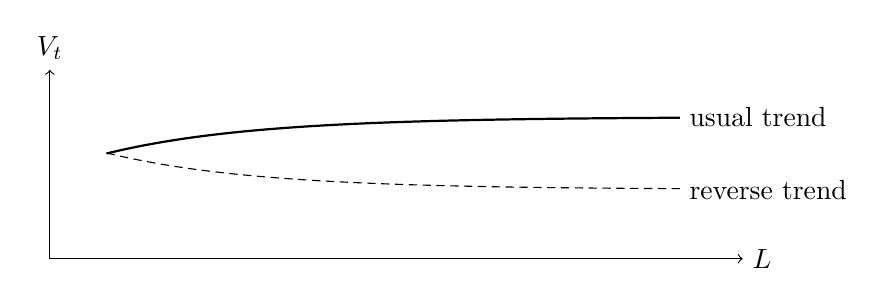
\begin{tikzpicture}[x=1.6cm,y=0.8cm]
 \draw[->] (0,0)--(5.5,0) node[right] {\(L\)};
 \draw[->] (0,0)--(0,3) node[above] {\(V_t\)};
 \draw[thick,domain=0.45:5,samples=60] plot (\x,{2.25-0.85*exp(-0.85*\x)});
 \draw[densely dashed,domain=0.45:5,samples=60] plot (\x,{1.1+0.85*exp(-0.85*\x)});
 \node[right] at (5,2.25) {usual trend};
 \node[right] at (5,1.1) {reverse trend};
\end{tikzpicture}
\end{latin}
\caption{طرح کیفی جهت تغییر آستانه با طول در دو رفتار توصیف‌شده در کتاب
و اسلاید ۲۰
\cite[بخش \secnum{۲.۴.۳.۳}]{weste}\cite{nonideal}.}
\label{fig:threshold-length-schematic}
\end{figure}

نام‌گذاری این قسمت از قرارداد کتاب برای وابستگی آستانه به طول پیروی
می‌کند. کتاب به کاربرد گسترده‌تر اصطلاح \lr{Short Channel Effect} برای
مجموعه اثرهای کانال کوتاه نیز اشاره می‌کند
\cite[پانوشت صفحه چاپی ۸۰]{weste}.

کتاب همچنین \lr{Narrow Channel Effect} را ذکر می‌کند که در آن آستانه
با عرض کانال تغییر می‌کند. اثر عرض معمولاً در مقایسه مورد بحث مرجع
کمتر است، زیرا حداقل عرض از حداقل طول بزرگ‌تر در نظر گرفته شده است
\cite[صفحه چاپی ۸۰]{weste}. مقدار و جهت وابستگی در یک افزاره مشخص به
ساختار و فرایند آن وابسته است.

با تغییر طول، ضریب \(\beta=\mu C_{\mathrm{ox}}W/L\) نیز تغییر می‌کند.
اگر مسئله، آستانه را تابع طول داده باشد، هم ضریب هندسی و هم
اضافه‌ولتاژ \(V_{GS}-V_t(L)\) باید به‌روزرسانی شوند.
در \lr{Channel Length Modulation} بخش \ref{sec:clm}، تغییر طول مؤثر
در اثر تغییر بایاس درین یک افزاره بررسی شد. در این قسمت، آستانه
افزاره‌ها با طول‌های مختلف مقایسه می‌شود.

در جدول \ref{tab:threshold-effects-summary} شرایط مقایسه سه اثر
گردآوری شده‌اند. علامت‌ها با قرارداد \lr{nMOS} بیان شده‌اند.
\begin{table}[!htbp]
\centering
\small
\caption{جهت تغییر آستانه در سه اثر این بخش، با ثابت بودن دیگر شرایط مقایسه.}
\label{tab:threshold-effects-summary}
\begin{tabularx}{\linewidth}{>{\raggedleft\arraybackslash}Xcc}
\toprule
اثر & متغیر مقایسه & نتیجه مدل\\
\midrule
\lr{Body Effect} & افزایش \(V_{SB}\) & افزایش \(V_t\)\\
\lr{DIBL} & افزایش \(V_{DS}\) & کاهش \(V_t\)\\
\lr{Short Channel Effect} معمول & کاهش \(L\) & کاهش \(V_t\)\\
رفتار \lr{Reverse Short Channel} & کاهش \(L\) & افزایش \(V_t\)\\
\bottomrule
\end{tabularx}
\end{table}

% !TeX root = booklet-02.tex
\subsection{جریان‌های نشتی}
\label{sec:leakage}
در افزاره واقعی، بایاس خاموش نیز با جریان‌های کوچکی همراه است. کتاب
سه مسیر اصلی را معرفی می‌کند. \lr{Subthreshold Leakage} در مسیر سورس
و درین، \lr{Gate Leakage} از راه عایق گیت و \lr{Junction Leakage} در
پیوندهای ناحیه‌های \lr{Diffusion} و بدنه جریان دارند
\cite[بخش \secnum{۲.۴.۴} و شکل \secnum{۲.۱۹}]{weste}
\cite[اسلایدهای ۲۱ و ۲۲]{nonideal}. بایاس، دما، هندسه و ساختار فرایند،
سهم هر مسیر را تعیین می‌کنند.

در روایت فناوری کتاب سال ۲۰۱۱، نشتی در نمونه‌های با ابعاد بالاتر از
\(\qty{180}{\nano\metre}\) معمولاً سهم کوچکی داشته است. برای نمونه‌های
\(\qty{90}{\nano\metre}\) و \(\qty{65}{\nano\metre}\)، جریان‌های
زیرآستانه در مرتبه یک تا چند ده نانوآمپر برای هر ترانزیستور گزارش
شده‌اند. در نمونه‌های \(\qty{45}{\nano\metre}\)، نازک‌شدن عایق، نشتی
گیت را نیز مهم می‌کند و مرجع نقش عایق‌های \lr{High-k} را مطرح می‌کند
\cite[صفحه ۸۱]{weste}. این اعداد به نمونه‌ها و زمان مرجع مربوط‌اند.

\subsubsection{\lr{Subthreshold Leakage}}
\label{sec:subthreshold-leakage}
\paragraph*{وارونگی ضعیف و معنای خاموشی}
در \lr{Weak Inversion}، ولتاژ گیت زیر آستانه است و مقدار جریان به‌صورت
نمایی با ولتاژ گیت تغییر می‌کند. در توصیف کتاب، عبور حرارتی حامل‌ها
از سد پتانسیل، جریان زیرآستانه را ایجاد می‌کند
\cite[بخش \secnum{۲.۴.۴.۱}]{weste}. در مدل سوئیچی، خروجی منطقی بر
اساس مسیرهای روشن و خاموش تحلیل می‌شود. مدل نشتی، مقدار جریان کوچک
مسیر خاموش و اثر آن بر توان و نگهداری بار را نیز محاسبه می‌کند.

\paragraph*{پیش‌نیاز تابع نمایی و لگاریتم ده‌دهی}
عدد \(e\approx2.71828\) پایه لگاریتم طبیعی است. تابع
\(\exp(x)=e^x\) برای هر \(x\) مثبت است. برای نمونه،
\(e^0=1\)، \(e^1\approx2.718\)، \(e^{-1}=1/e\approx0.368\) و
\(e^{-3}\approx0.0498\). منفی‌ترشدن توان، مقدار تابع را کوچک‌تر می‌کند.
قانون \(e^{a+b}=e^ae^b\) و در نتیجه \(e^a/e^b=e^{a-b}\) در محاسبه
نسبت نشتی‌ها به کار می‌روند.

لگاریتم ده‌دهی \(\log_{10}x\)، توانی از ده است که عدد \(x>0\) را
می‌سازد. مثلاً \(\log_{10}1000=3\) و \(\log_{10}0.01=-2\).
یک \lr{Decade} تغییر جریان یعنی ضرب یا تقسیم آن در ده.
برای تبدیل پایه از رابطه \(\log_{10}x=\ln x/\ln10\) استفاده می‌کنیم.
همچنین \(e^x=10^{x/\ln10}\) است. نسبت‌های داخل لگاریتم و توان تابع
نمایی باید بی‌بعد باشند.

\paragraph*{مدل جریان و تعریف همه پارامترها}
رابطه \secnum{۲.۴۲} کتاب و اسلاید ۲۳ برای \lr{nMOS} با
\(V_{DS}\ge0\) چنین بازنویسی می‌شود
\begin{equation}
 I_{\mathrm{sub}}=I_{ds0}
 \exp\!\left(\frac{V_{GS}-V_{t0}+\eta V_{DS}-k_\gamma V_{SB}}{nv_T}\right)
 \left(1-e^{-V_{DS}/v_T}\right).
 \label{eq:leakage-subthreshold-model}
\end{equation}
در این رابطه، \(V_{t0}\) آستانه مرجع، \(\eta\) ضریب \lr{DIBL} و
\(k_\gamma\) ضریب خطی اثر بدنه از
\eqref{eq:body-linearization} هستند. \(n>0\) ضریب وابسته به فرایند
است که مرجع مقدار معمول آن را حدود \num{1.3} تا \num{1.7} می‌گیرد.
\(v_T=kT/q\) ولتاژ حرارتی است. \(I_{ds0}\) ضریب جریان وابسته به
فرایند و هندسه است \cite[صفحات ۸۱ و ۸۲]{weste}.

صورت کسر داخل نمایی، یک ولتاژ است. مخرج \(nv_T\) نیز ولتاژ است، پس
توان بی‌بعد می‌شود. عامل آخر هم بی‌بعد است و واحد کل جریان از
\(I_{ds0}\) به دست می‌آید. برای استفاده از آستانه مؤثر، می‌توان
\(V_{t,\mathrm{eff}}=V_{t0}-\eta V_{DS}+k_\gamma V_{SB}\) را تعریف کرد
و صورت توان را \(V_{GS}-V_{t,\mathrm{eff}}\) نوشت.
این صورت از تقریب خطی بایاس بدنه استفاده می‌کند و دامنه آن با
\eqref{eq:body-linear-error} سنجیده می‌شود.

مدل مرجع، ضریب جریان را با رابطه تجربی زیر نیز تقریب می‌زند
\begin{equation}
 I_{ds0}=\beta v_T^2e^{1.8},\qquad
 \beta=\mu C_{\mathrm{ox}}\frac{W}{L}.
 \label{eq:leakage-current-prefactor}
\end{equation}
عدد \(1.8\) ضریب تجربی همان مدل است
\cite[رابطه \secnum{۲.۴۳}]{weste}. حاصل‌ضرب
\(\beta\) با واحد \(\unit{\ampere\per\volt\squared}\) و \(v_T^2\)،
واحد آمپر دارد. در شرایطی که صورت توان صفر و
\(V_{DS}\gg v_T\) باشد، جریان به \(I_{ds0}\) نزدیک می‌شود.
پارامترهای این رابطه می‌توانند با دما و فرایند تغییر کنند.

\paragraph*{عامل درین و معیار تقریب آن}
برای بررسی عامل آخر، \(D=V_{DS}\) و
\(F(D)=1-e^{-D/v_T}\) را تعریف می‌کنیم. در \(D=0\)، عامل \(F\)
صفر و جریان مدل نیز صفر است. با افزایش \(D>0\)، این عامل به یک
نزدیک می‌شود. چند مقدار در جدول \ref{tab:leakage-drain-factor}
آمده‌اند.
\begin{table}[!htbp]
\centering
\small
\caption{عامل درین در مدل زیرآستانه و فاصله نسبی آن از یک.}
\label{tab:leakage-drain-factor}
\begin{tabular}{cccc}
\toprule
\(D/v_T\) & \(e^{-D/v_T}\) & \(F(D)\) & فاصله از یک، درصد\\
\midrule
\num{1} & \num{0.3679} & \num{0.6321} & \num{36.79}\\
\num{2} & \num{0.1353} & \num{0.8647} & \num{13.53}\\
\num{3} & \num{0.0498} & \num{0.9502} & \num{4.98}\\
\num{5} & \num{0.00674} & \num{0.99326} & \num{0.674}\\
\bottomrule
\end{tabular}
\end{table}

برای فاصله حداکثر ۱ درصد از یک، باید
\(e^{-D/v_T}\le0.01\) باشد. با لگاریتم‌گیری،
\(D\ge-v_T\ln0.01\approx4.605v_T\) به دست می‌آید.
در \(v_T=\qty{26}{\milli\volt}\)، این شرط حدود
\(D\ge\qty{120}{\milli\volt}\) است. در
\(D=\qty{50}{\milli\volt}\)، عامل برابر \(0.8538\) و در
\(D=\qty{100}{\milli\volt}\)، برابر \(0.9786\) است.
در استفاده از تعبیر «چند برابر ولتاژ حرارتی» در متن مرجع، دقت مورد
نیاز محاسبه تعیین‌کننده انتخاب تقریب است.

در \(D\ll v_T\)، تقریب \(e^{-D/v_T}\approx1-D/v_T\) می‌دهد
\(F(D)\approx D/v_T\). ازاین‌رو، جریان در نزدیکی درین صفر با
\(D\) متناسب می‌شود. در \(D\gg v_T\)، عامل \(F\) تقریباً ثابت
است، اما جمله \(\eta D\) در توان هنوز می‌تواند با افزایش درین،
نشتی را افزایش دهد.

\paragraph*{مثال آموزشی مقدار جریان و اثر گیت}
فرض کنید \(\beta=\qty{1}{\milli\ampere\per\volt\squared}\)،
\(n=1.4\)، \(v_T=\qty{0.026}{\volt}\)،
\(V_{t0}=\qty{0.35}{\volt}\)، \(\eta=0.05\)،
\(V_{DS}=\qty{1}{\volt}\) و \(V_{SB}=0\) باشند.
این پارامترها برای یک مثال آموزشی فرض شده‌اند. ابتدا داریم
\begin{equation}
 I_{ds0}=(10^{-3})(0.026)^2e^{1.8}\,\unit{\ampere}
 \approx\qty{4.090}{\micro\ampere}.
 \label{eq:leakage-prefactor-example}
\end{equation}
در \(V_{GS}=0\)، صورت توان
\(-0.35+0.05(1)=-\qty{0.30}{\volt}\) و مخرج
\(1.4(0.026)=\qty{0.0364}{\volt}\) است.
چون \(F(\qty{1}{\volt})\approx1\)، جریان برابر است با
\begin{equation}
 I_{\mathrm{off}}\approx(4.090\times10^{-6})e^{-0.30/0.0364}
 \approx\qty{1.077}{\nano\ampere}.
 \label{eq:leakage-absolute-example}
\end{equation}
اگر فقط گیت به \(\qty{0.1}{\volt}\) برسد، نسبت دو جریان از قانون
تقسیم توابع نمایی به دست می‌آید
\begin{equation}
 \frac{I(\qty{0.1}{\volt})}{I(0)}
 =e^{0.1/0.0364}\approx15.60,
 \qquad I(\qty{0.1}{\volt})\approx\qty{16.81}{\nano\ampere}.
 \label{eq:leakage-gate-ratio-example}
\end{equation}
آستانه مؤثر در هر دو نقطه \(\qty{0.30}{\volt}\) است و هر دو بایاس
گیت در دامنه زیرآستانه قرار دارند.

\paragraph*{استخراج \lr{Subthreshold Slope} و خواندن نمودار لگاریتمی}
در بایاس درین، بدنه و دمای ثابت، تمام عامل‌های مستقل از گیت را در یک
ضریب ثابت جمع می‌کنیم. برای یک جریان مرجع ثابت \(I_r>0\)، از
\eqref{eq:leakage-subthreshold-model} نتیجه می‌شود
\begin{equation}
 y=\log_{10}\!\left(\frac{I_{\mathrm{sub}}}{I_r}\right)
 =c+\frac{V_{GS}}{nv_T\ln10}.
 \label{eq:leakage-log-line}
\end{equation}
نماد \(c\) یک مقدار ثابت در این مقایسه است. پس نمودار \(y\) برحسب
\(V_{GS}\) خطی است و شیب آن \(1/(nv_T\ln10)\) می‌شود.
کتاب معکوس این شیب را \lr{Subthreshold Slope} می‌نامد
\begin{equation}
 \boxed{S=\left[\frac{\mathrm{d}\log_{10}(I_{\mathrm{sub}}/I_r)}
 {\mathrm{d}V_{GS}}\right]^{-1}=nv_T\ln10}.
 \label{eq:leakage-subthreshold-slope}
\end{equation}
این رابطه با \secnum{۲.۴۴} کتاب و اسلاید ۲۳ متناظر است
\cite{weste,nonideal}. \(S\) تغییر گیت لازم برای ده‌برابرشدن جریان
است و معمولاً با واحد \(\unit{\milli\volt}\) به ازای یک
\lr{Decade} بیان می‌شود. در مثال قبل،
\(S=1.4(0.026)\ln10\approx\qty{83.81}{\milli\volt}\) است.
افزایش گیت به اندازه \(2S\)، جریان را صد برابر می‌کند.

شکل \ref{fig:leakage-semilog} نسبت جریان به مقدار گیت صفر را برای
همین \(S\) نشان می‌دهد. فاصله برابر روی محور عمودی لگاریتمی، به معنای
ضریب برابر در جریان است. برای \(n\) بین \num{1.3} و \num{1.7} و
\(v_T=\qty{26}{\milli\volt}\)، مقدار \(S\) حدود
\(\qty{77.8}{\milli\volt}\) تا \(\qty{101.8}{\milli\volt}\) به ازای هر دهه است.
\begin{figure}[!htbp]
\centering
\begin{latin}
\PersianMathDigits
\begin{tikzpicture}[x=22cm,y=1.05cm]
 \draw[->] (-0.12,-1.5)--(0.24,-1.5) node[right] {\(V_{GS}\;(\mathrm{V})\)};
 \draw[->] (-0.12,-1.5)--(-0.12,2.8) node[above] {\(I/I_{\mathrm{off}}\)};
 \foreach \x in {-0.1,0,0.1,0.2} {\draw (\x,-1.5)--(\x,-1.56) node[below] {\(\x\)};}
 \foreach \y/\value in {-1/0.1,0/1,1/10,2/100} {
  \draw (-0.12,\y)--(-0.125,\y) node[left] {\(\value\)};
 }
 \draw[thick,domain=-0.1:0.2,samples=50] plot (\x,{\x/0.0838141});
 \draw[dotted] (0,0)--(0.0838141,0)--(0.0838141,1)--(0,1);
 \draw[<->] (0,0.15)--(0.0838141,0.15) node[midway,above] {\(S\)};
\end{tikzpicture}
\end{latin}
\caption{نمودار آموزشی زیرآستانه با محور عمودی لگاریتمی و
\(S=\qty{83.81}{\milli\volt}\) به ازای هر دهه. گیت به اندازه \(S\)
تغییر می‌کند و نسبت جریان از یک به ده می‌رسد. بایاس‌های دیگر ثابت‌اند.}
\label{fig:leakage-semilog}
\end{figure}

در شکل \secnum{۲.۲۰} کتاب، محور عمودی جریان بر واحد عرض با واحد
\(\unit{\ampere\per\micro\metre}\) است. برای نمونه
\(\qty{65}{\nano\metre}\) در دمای \(\qty{70}{\degreeCelsius}\)،
مقادیر حدود \(\qty{27}{\nano\ampere\per\micro\metre}\) و
\(\qty{2}{\nano\ampere\per\micro\metre}\) در گیت صفر و دو بایاس
درین \(\qty{1.0}{\volt}\) و \(\qty{0.1}{\volt}\) مشخص شده‌اند.
نسبت آن‌ها حدود \(13.5\) است. بخش تقریباً خطی منحنی زیرآستانه و
بالارفتن جریان در گیت بسیار منفی، به‌ترتیب رفتار نمایی و اثر
\lr{GIDL} را نشان می‌دهند \cite[صفحه ۸۱]{weste}.

\paragraph*{بازنویسی دقیق نسبت به \(I_{\mathrm{off}}\)}
جریان مرجع را در گیت و بایاس بدنه صفر و درین \(V_{DD}>0\) تعریف
می‌کنیم. از \eqref{eq:leakage-subthreshold-model} داریم
\begin{equation}
 I_{\mathrm{off}}=I_{ds0}
 e^{(-V_{t0}+\eta V_{DD})/(nv_T)}F(V_{DD}).
 \label{eq:leakage-off-definition}
\end{equation}
تقسیم رابطه جریان بر رابطه مرجع، عامل \(I_{ds0}\) و آستانه مرجع را
حذف می‌کند. با استفاده از \(S=nv_T\ln10\)، نتیجه برابر است با
\begin{equation}
 \boxed{I_{\mathrm{sub}}=I_{\mathrm{off}}
 10^{[V_{GS}+\eta(V_{DS}-V_{DD})-k_\gamma V_{SB}]/S}
 \frac{F(V_{DS})}{F(V_{DD})}}.
 \label{eq:leakage-off-normalized}
\end{equation}
در بایاس مرجع، توان صفر و نسبت دو عامل \(F\) برابر یک است و جریان
مرجع دقیقاً بازیابی می‌شود. در بازنویسی رابطه \secnum{۲.۴۵} کتاب،
عامل مخرج با فرض \(V_{DD}\gg v_T\) تقریباً یک گرفته شده است.
برای نگه‌داشتن همه عامل‌ها در بایاس درین کوچک، از
\eqref{eq:leakage-off-normalized} استفاده می‌کنیم.

این نسبت برای هندسه، دما و پارامترهای یکسان نوشته شده است.
در یک دمای ثابت، افزایش \(V_{t0}\) به اندازه \(\Delta V_t>0\)،
جریان را در عامل \(e^{-\Delta V_t/(nv_T)}\) ضرب می‌کند.
افزایش بایاس بدنه در تقریب خطی، عامل
\(e^{-k_\gamma\Delta V_{SB}/(nv_T)}\) و تغییر درین، هم عامل نمایی
\lr{DIBL} و هم نسبت دو \(F\) را وارد می‌کند.
برای \lr{pMOS} با قرارداد بزرگی‌های مثبت، همین ساختار با
\(V_{SG},V_{SD},V_{BS}\)، بزرگی آستانه و پارامترهای آن افزاره به کار
می‌رود.

\paragraph*{حل مثال \secnum{۲.۶} کتاب و نسبت هزاربرابری}
مثال مرجع می‌خواهد جریان گیت صفر، هزار برابر کوچک‌تر از جریان در
گیت برابر آستانه باشد. در یک بایاس درین ثابت با \(V_{DS}\gg v_T\)،
بایاس بدنه صفر و با قرارداد آستانه همان مقایسه، نسبت جریان‌ها چنین است
\begin{equation}
 \frac{I(0)}{I(V_t)}=e^{-V_t/(nv_T)}=10^{-3}.
 \label{eq:leakage-three-decades}
\end{equation}
از دو طرف لگاریتم می‌گیریم. با \(\ln10^{-3}=-3\ln10\)، داریم
\begin{equation}
 -\frac{V_t}{nv_T}=-3\ln10
 \quad\Longrightarrow\quad V_t=3nv_T\ln10=3S.
 \label{eq:leakage-minimum-threshold}
\end{equation}
پس برای \(n=1.5\) و \(v_T=\qty{26}{\milli\volt}\)،
\(S\approx\qty{89.8}{\milli\volt}\) و
\(V_t\approx\qty{269.4}{\milli\volt}\) است. گردکردن مرجع حدود
\(\qty{270}{\milli\volt}\) می‌دهد. برای نمونه \lr{Silicon-on-Insulator
(SOI)} مثال با \(n=1.3\)، مقدار \(S\approx\qty{77.8}{\milli\volt}\)
و \(V_t\approx\qty{233.5}{\milli\volt}\) می‌شود
\cite[مثال \secnum{۲.۶}، صفحه ۸۲]{weste}.
شرط حداقل آستانه برای نسبت حداکثر \(10^{-3}\)، همان
\(V_t\ge3S\) است.

\paragraph*{اثر بر توان و نگهداری بار}
توان ایستای دریافت‌شده از یک منبع ثابت از
\(P_{\mathrm{static}}=V_{DD}I_{\mathrm{supply}}\) به دست می‌آید.
در یک مثال فرضی با \(10^8\) ترانزیستور، کسر خاموش \(0.8\)، نشتی
متوسط هر ترانزیستور خاموش \(\qty{1}{\nano\ampere}\) و تغذیه
\(\qty{1}{\volt}\)، اگر این جریان‌ها سهم جمع‌پذیر همان منبع باشند،
جریان کل \(\qty{0.08}{\ampere}\) و توان \(\qty{80}{\milli\watt}\)
می‌شود. برای مدار مشخص، اتصال مسیرها و جریان دریافتی از هر منبع با
\lr{KCL} محاسبه می‌شود.

نشتی همچنین بار گره خازنی را در طول زمان تغییر می‌دهد. با جریان
تقریباً ثابت \(I\)، تغییر ولتاژ \(\Delta V\) روی ظرفیت \(C\) در زمان
\(t\approx C\Delta V/I\) رخ می‌دهد. مثلاً
\(C=\qty{10}{\femto\farad}\)، \(I=\qty{1}{\nano\ampere}\) و
\(\Delta V=\qty{0.2}{\volt}\)، زمان حدود \(\qty{2}{\micro\second}\)
می‌دهند. این برآورد آموزشی، حساسیت گره‌های ذخیره بار و نیاز به
\lr{Refresh} در حافظه پویا را توضیح می‌دهد
\cite[صفحه ۸۲]{weste}.

\subsubsection{\lr{Gate Leakage}}
\label{sec:gate-leakage}
\paragraph*{تونل‌زنی و دو سازوکار مرجع}
در عایق بسیار نازک، احتمال عبور کوانتومی حامل از سد عایق، جریان
تونل‌زنی ایجاد می‌کند. برای بیان مقیاس، کتاب عایق‌های نازک‌تر از حدود
\(\qty{1.5}{\nano\metre}\) تا \(\qty{2.0}{\nano\metre}\) را در این
بحث مطرح می‌کند. کتاب دو سازوکار \lr{Fowler-Nordheim (FN)
Tunneling} و \lr{Direct Tunneling} را معرفی می‌کند.
اولی در ولتاژ زیاد و ضخامت متوسط اهمیت پیدا می‌کند و در برنامه‌ریزی
\lr{EEPROM} به کار می‌رود. دومی در عایق نازک و ولتاژ پایین‌تر اهمیت
دارد \cite[بخش \secnum{۲.۴.۴.۲}]{weste}.

برای \lr{Direct Tunneling}، رابطه \secnum{۲.۴۷} کتاب و اسلاید ۲۴ را
با نام‌گذاری ضرایب مستقل می‌نویسیم
\begin{equation}
 I_{\mathrm{gate}}=WA_g
 \left(\frac{V_{DD}}{t_{\mathrm{ox}}}\right)^2
 \exp\!\left(-B_g\frac{t_{\mathrm{ox}}}{V_{DD}}\right).
 \label{eq:gate-tunneling-model}
\end{equation}
\(A_g,B_g\) همان ثابت‌های فناوری \(A,B\) در مرجع هستند.
زیرنویس‌ها برای تشخیص آن‌ها از ضرایب مدل پیوند به کار رفته‌اند.
\(W\) عرض و \(t_{\mathrm{ox}}\) ضخامت فیزیکی عایق در مدل است.
این مدل تجربی در شرایط بایاس و پارامترهای مربوط به برازش استفاده
می‌شود \cite[صفحه ۸۳]{weste}\cite[اسلاید ۲۴]{nonideal}.

با دستگاه طول متر، بی‌بعدبودن توان ایجاب می‌کند
\([B_g]=\unit{\volt\per\metre}\). چون
\(W(V_{DD}/t_{\mathrm{ox}})^2\) واحد
\(\mathrm{V}^2/\mathrm{m}\) دارد،
\([A_g]=\mathrm{A\,m\,V^{-2}}\) است. اگر ضرایب با نانومتر برازش
شده‌اند، ضخامت و واحد ضرایب نیز با همان قرارداد وارد می‌شوند.

\paragraph*{حساسیت ضخامت و مثال نسبت جریان}
در ولتاژ، عرض و ضرایب ثابت، برای دو ضخامت مثبت \(t_1,t_2\)، تقسیم
دو رابطه \eqref{eq:gate-tunneling-model} می‌دهد
\begin{equation}
 \frac{I_2}{I_1}=\left(\frac{t_1}{t_2}\right)^2
 \exp\!\left[\frac{B_g(t_1-t_2)}{V_{DD}}\right].
 \label{eq:gate-thickness-ratio}
\end{equation}
کاهش ضخامت، هم عامل مربعی و هم عامل نمایی را افزایش می‌دهد.
در مثال فرضی \(t_1=\qty{1.1}{\nano\metre}\)،
\(t_2=\qty{1.0}{\nano\metre}\)، \(V_{DD}=\qty{1}{\volt}\) و
\(B_g=\qty{10}{\volt\per\nano\metre}\)، نسبت برابر
\((1.1/1.0)^2e^1\approx3.29\) است. مقدار \(B_g\) در این مثال
آموزشی فرض شده است. برای جریان مطلق، مقدار \(A_g\) نیز لازم است.
با ثابت بودن دیگر پارامترها، دوبرابرشدن عرض در همین مدل جریان را
دو برابر می‌کند.

در متن مرجع، برای داده‌های مورد بحث، افزایش جریان حداقل با ضریب
حدود \(2.7\) به ازای کاهش یک آنگستروم ضخامت گزارش شده است.
کتاب مقیاس ضخامت \(\qty{1.05}{\nano\metre}\)، معادل \num{10.5} آنگستروم، و چگالی جریان
\(\qty{100}{\ampere\per\centi\metre\squared}\) و ضخامت حدود
\(\qty{0.3}{\nano\metre}\) برای هر لایه اتمی \lr{SiO2} را در توضیح
نمونه‌های همان دوره مطرح می‌کند \cite[صفحه ۸۳]{weste}.
این اعداد همراه ماده و شرایط نمودار مرجع تفسیر می‌شوند.

\paragraph*{ولتاژ، چگالی جریان و عایق \lr{High-k}}
در ضخامت ثابت، نسبت جریان در دو ولتاژ مثبت چنین است
\begin{equation}
 \frac{I(V_2)}{I(V_1)}=
 \left(\frac{V_2}{V_1}\right)^2
 \exp\!\left[B_gt_{\mathrm{ox}}
 \left(\frac{1}{V_1}-\frac{1}{V_2}\right)\right].
 \label{eq:gate-voltage-ratio}
\end{equation}
برای \(V_2>V_1\)، هر دو عامل نسبت را افزایش می‌دهند.
در شکل \secnum{۲.۲۱} کتاب، محور عمودی چگالی جریان گیت
\(J_G=I_{\mathrm{gate}}/A_{\mathrm{gate}}\) با واحد
\(\unit{\ampere\per\centi\metre\squared}\) است.
برای چگالی یکنواخت، جریان از ضرب چگالی در مساحت به دست می‌آید.
مثلاً \(J_G=\qty{1}{\ampere\per\centi\metre\squared}\) و مساحت
فرضی \(\qty{0.005}{\micro\metre\squared}
=\qty{5e-11}{\centi\metre\squared}\)، جریان
\(\qty{50}{\pico\ampere}\) می‌دهند.
در شکل زیرآستانه \secnum{۲.۲۰}، نرمال‌سازی با عرض انجام شده است.
واحد محور هر شکل، نحوه تبدیل به جریان کل را تعیین می‌کند.

برای جریان روشن زیاد، ظرفیت اکسید بر واحد سطح بزرگ مطلوب است.
از \(C_{\mathrm{ox}}=\varepsilon/t\)، افزایش \lr{Permittivity} عایق
امکان استفاده از ضخامت فیزیکی بیشتر را در ظرفیت یکسان فراهم می‌کند.
ضخامت معادل اکسید از \(\mathrm{EOT}=t\varepsilon_{\mathrm{ox}}/
\varepsilon\) به دست می‌آید. تونل‌زنی به ضخامت فیزیکی و ویژگی سد
ماده وابسته است، پس ضرایب نشتی نیز باید با ماده عایق سازگار باشند.
در نمونه‌های \lr{SiO2} مورد بحث کتاب، نشتی گیت \lr{nMOS} می‌تواند
در مرتبه ده برابر \lr{pMOS} باشد، زیرا حامل‌ها سدهای انرژی متفاوتی
دارند. مرجع وابستگی این رفتار به نوع عایق را یادآور می‌شود
\cite[صفحه ۸۳]{weste}.

\subsubsection{\lr{Junction Leakage}}
\label{sec:junction-leakage}
\paragraph*{مدل دیود و علامت ولتاژ پیوند}
پیوند ناحیه‌های \lr{Diffusion} با بدنه یا \lr{Well} و پیوند
\lr{Well} با \lr{Substrate} مانند دیود عمل می‌کنند.
در بایاس معمول، بدنه و \lr{Well} به زمین یا تغذیه متصل می‌شوند تا
پیوندها در بایاس صفر یا معکوس قرار گیرند
\cite[بخش \secnum{۲.۴.۴.۳} و شکل \secnum{۲.۲۲}]{weste}.
مدل دیود کتاب را با نماد \(I_{\mathrm{dio}}\) برای جریان و
\(I_{\mathrm{rev}}>0\) برای ضریب جریان معکوس بازنویسی می‌کنیم
\begin{equation}
 I_{\mathrm{dio}}=I_{\mathrm{rev}}
 \left(e^{V_{\mathrm{dio}}/v_T}-1\right),\qquad
 V_{\mathrm{dio}}=V_{\mathrm{anode}}-V_{\mathrm{cathode}}.
 \label{eq:junction-diode-model}
\end{equation}
این دو جریان با \(I_D,I_S\) رابطه \secnum{۲.۴۸} کتاب متناظرند.
نمادهای مرجع در این رابطه به جریان دیود و ضریب جریان معکوس اشاره
دارند \cite[صفحه ۸۴ و پانوشت آن]{weste}\cite[اسلاید ۲۶]{nonideal}.

در پیوند \lr{nMOS}، بدنه \lr{p-type} آند و ناحیه
\lr{n-type Diffusion} کاتد است. بنابراین برای پیوند درین و بدنه،
\(V_{\mathrm{dio}}=V_B-V_D=-V_{DB}\) است.
اگر \(V_{DB}>0\)، ولتاژ دیود منفی و جریان آن در قرارداد آند به
کاتد منفی می‌شود. در بایاس معکوس بزرگ‌تر از چند برابر \(v_T\)،
جمله نمایی به صفر نزدیک و
\(I_{\mathrm{dio}}\approx-I_{\mathrm{rev}}\) است.
جریان معکوس در این قرارداد از ناحیه درین به بدنه می‌رود.
در بایاس صفر نیز \(I_{\mathrm{dio}}=0\) حاصل می‌شود.

ضریب \(I_{\mathrm{rev}}\) به ناخالصی، مساحت و محیط ناحیه
\lr{Diffusion} وابسته است. کتاب برای مؤلفه معمول دیود، مرتبه
\(\qty{0.01}{\femto\ampere\per\micro\metre\squared}\) تا
\(\qty{0.1}{\femto\ampere\per\micro\metre\squared}\) را در
نمونه‌های مورد بحث ذکر می‌کند \cite[صفحه ۸۴]{weste}.
در مثال فرضی با چگالی \(\qty{0.1}{\femto\ampere\per\micro\metre\squared}\)،
مساحت \(\qty{0.2}{\micro\metre\squared}\) و صرف‌نظر از سهم محیط،
\(I_{\mathrm{rev}}=\qty{0.02}{\femto\ampere}\) می‌شود.
در بایاس معکوس \(\qty{1}{\volt}\) و
\(v_T=\qty{0.026}{\volt}\)، جریان حدود
\(-\qty{0.02}{\femto\ampere}\) است.

\paragraph*{\lr{Band-to-Band Tunneling} و نقش ناخالصی}
در پیوندهای با ناخالصی زیاد، میدان قوی می‌تواند
\lr{Band-to-Band Tunneling (BTBT)} ایجاد کند.
مرجع اثر \lr{Halo Doping}، یعنی افزایش ناخالصی نزدیک انتهای کانال
برای کنترل آستانه، را بر افزایش این نشتی توضیح می‌دهد.
وجود تله‌های ناشی از نقص ماده نیز می‌تواند
\lr{Trap-Assisted Tunneling (TAT)} را تقویت کند.
در توصیف کتاب، سهم مهمی از این جریان نزدیک دیواره پیوند رو به
کانال رخ می‌دهد \cite[صفحه ۸۴]{weste}\cite[اسلاید ۲۷]{nonideal}.

رابطه تجربی \secnum{۲.۴۹} کتاب برای بزرگی جریان چنین است
\begin{equation}
 I_{\mathrm{BTBT}}=WX_j A_b\frac{E_j}{E_g^{1/2}}V_{DD}
 \exp\!\left(-B_b\frac{E_g^{3/2}}{E_j}\right).
 \label{eq:junction-btbt-model}
\end{equation}
\(X_j\) عمق پیوند، \(E_j\) بزرگی میدان پیوند و \(A_b,B_b\)
ثابت‌های فناوری هستند. کتاب \(E_g\) را ولتاژ متناظر با گاف انرژی
تعریف می‌کند. اگر انرژی گاف برحسب ژول معلوم باشد، تقسیم آن بر
\(q\) مقدار \(E_g\) را برحسب ولت می‌دهد.
توان‌های \(1/2\) و \(3/2\) روی همین کمیت اعمال می‌شوند.
در قرارداد طول متر، بی‌بعدبودن توان و واحد آمپر نتیجه می‌دهند
\begin{equation}
 [B_b]=\mathrm{m}^{-1}\mathrm{V}^{-1/2},\qquad
 [A_b]=\mathrm{A\,m}^{-1}\mathrm{V}^{-3/2}.
 \label{eq:junction-btbt-units}
\end{equation}
ضرایب \(A_b,B_b\) با \(A_g,B_g\) مدل گیت جداگانه تعریف و برازش
می‌شوند.

\paragraph*{میدان پیوند و یک محاسبه آموزشی}
در بایاس معکوس \(V_{DD}\)، رابطه \secnum{۲.۵۰} کتاب میدان را با
ناخالصی \lr{Halo} و \lr{Source/Drain} مرتبط می‌کند
\begin{equation}
 E_j=\sqrt{\frac{2qN_{\mathrm{halo}}N_{\mathrm{sd}}}
 {\varepsilon_{\mathrm{si}}(N_{\mathrm{halo}}+N_{\mathrm{sd}})}
 \left[V_{DD}+v_T\ln\!\left(
 \frac{N_{\mathrm{halo}}N_{\mathrm{sd}}}{n_i^2}\right)\right]}.
 \label{eq:junction-field-model}
\end{equation}
همه غلظت‌ها باید با واحد یکسان و \(\varepsilon_{\mathrm{si}}\) با
واحد طول سازگار وارد شوند. برای دنبال‌کردن محاسبه،
دو کمیت کمکی را تعریف می‌کنیم
\begin{equation}
 N_{\mathrm{eff}}=\frac{N_{\mathrm{halo}}N_{\mathrm{sd}}}
 {N_{\mathrm{halo}}+N_{\mathrm{sd}}},\qquad
 \phi_{\mathrm{bi}}=v_T\ln\!\left(
 \frac{N_{\mathrm{halo}}N_{\mathrm{sd}}}{n_i^2}\right).
 \label{eq:junction-field-parameters}
\end{equation}
با جایگذاری آن‌ها، رابطه میدان به شکل ساده‌تر زیر تبدیل می‌شود
\[
 E_j=\sqrt{\frac{2qN_{\mathrm{eff}}}{\varepsilon_{\mathrm{si}}}
 (V_{DD}+\phi_{\mathrm{bi}})}.
\]
\(\phi_{\mathrm{bi}}\) واحد ولت دارد و عبارت زیر رادیکال، واحد
\(\mathrm{V}^2/\mathrm{m}^2\) یا شکل سازگار سانتی‌متری آن را دارد.

در مثال فرضی، \(N_{\mathrm{halo}}=\qty{e18}{\per\centi\metre\cubed}\)،
\(N_{\mathrm{sd}}=\qty{e20}{\per\centi\metre\cubed}\)،
\(n_i=\qty{1.45e10}{\per\centi\metre\cubed}\)،
\(v_T=\qty{0.026}{\volt}\) و
\(\varepsilon_{\mathrm{si}}=11.7(\qty{8.85e-14}{\farad\per\centi\metre})\)
هستند. محاسبه می‌دهد
\begin{align}
 N_{\mathrm{eff}}&\approx\qty{9.901e17}{\per\centi\metre\cubed},
 &\phi_{\mathrm{bi}}&\approx\qty{1.0583}{\volt},\notag\\
 E_j(V_{DD}=\qty{0.8}{\volt})&\approx\qty{7.541e5}{\volt\per\centi\metre},
 &E_j(V_{DD}=\qty{1.2}{\volt})&\approx\qty{8.313e5}{\volt\per\centi\metre}.
 \label{eq:junction-field-example}
\end{align}
برای مشاهده حساسیت نمایی، حاصل‌ضرب فرضی
\(B_bE_g^{3/2}=\qty{3e6}{\volt\per\centi\metre}\) را ثابت می‌گیریم.
تقسیم دو جریان \eqref{eq:junction-btbt-model} با هندسه و گاف یکسان
می‌دهد
\begin{equation}
 \frac{I_2}{I_1}=
 \frac{1.2}{0.8}\frac{E_{j2}}{E_{j1}}
 \exp\!\left[3\times10^6
 \left(\frac{1}{E_{j1}}-\frac{1}{E_{j2}}\right)\right]
 \approx2.39.
 \label{eq:junction-btbt-ratio-example}
\end{equation}
در این جایگذاری عددی، میدان‌ها برحسب
\(\unit{\volt\per\centi\metre}\) وارد شده‌اند.
برای جریان مطلق، ثابت \(A_b\) و دیگر پارامترهای همان فناوری لازم‌اند.

\paragraph*{\lr{Gate-Induced Drain Leakage}}
\lr{Gate-Induced Drain Leakage (GIDL)} نزدیک ناحیه هم‌پوشانی گیت و
درین رخ می‌دهد. درین بالا و گیت پایین، میدان این ناحیه را تقویت
می‌کنند. در \lr{nMOS}، منفی‌ترکردن گیت در درین بالا می‌تواند این
مسیر را شدیدتر کند. جریان به ناحیه هم‌پوشانی و در نتیجه به عرض
افزاره وابسته است \cite[صفحات ۸۴ و ابتدای ۸۵]{weste}
\cite[اسلاید ۲۸]{nonideal}.
در توصیف نمونه‌های کتاب، سهم این مسیر در
\(|V_{GD}|\le V_{DD}\) معمولاً کوچک است و با راندن گیت بیرون ریل
تغذیه برجسته می‌شود.

برای مثال، در \(V_D=\qty{1}{\volt}\)، تغییر گیت از صفر به
\(-\qty{0.3}{\volt}\)، ولتاژ \(V_{DG}=V_D-V_G\) را از
\(\qty{1}{\volt}\) به \(\qty{1.3}{\volt}\) می‌رساند.
در مدل زیرآستانه، گیت منفی جریان سورس و درین را کاهش می‌دهد، اما
میدان درین و گیت در همین تغییر افزایش می‌یابد.
شکل \secnum{۲.۲۰} کتاب بالا رفتن جریان در سمت گیت منفی را نشان
می‌دهد. برای محاسبه کل نشتی در آن بایاس، همه مسیرهای مربوط به
بایاس و جریان دریافتی از منبع باید در مدل مدار لحاظ شوند.

% !TeX root = booklet-02.tex
\clearpage
\subsection{وابستگی به دما}
\label{sec:temperature-dependence}
افزایش دما، هم حرکت حامل‌ها و هم ولتاژ آستانه را تغییر می‌دهد. برای
محاسبه جریان، باید این تغییرها را هم‌زمان وارد مدل کرد
\cite[بخش \secnum{۲.۴.۵}، صفحات ۸۵ و ۸۶]{weste}
\cite[اسلاید ۲۹]{nonideal}. در این بخش، \(T\) دمای مطلق، \(T_r\)
دمای مرجع و \(\mu\) همان \lr{Mobility} مورد استفاده در مدل جریان است.

\subsubsection*{دمای مطلق، توان منفی و کاهش \lr{Mobility}}
ارتباط دمای سلسیوس \(t_C\) با دمای مطلق به صورت زیر است.
\[
 T/\unit{\kelvin}=t_C/\unit{\degreeCelsius}+273.15.
\]
مثلاً \(\qty{300}{\kelvin}\) برابر \(\qty{26.85}{\degreeCelsius}\)
است. اختلاف دمای یک کلوین با اختلاف یک درجه سلسیوس برابر است.
در نسبت دماها باید مقدار کلوین را به کار برد. نسبت دماهای سلسیوس
معنای مورد نیاز رابطه \eqref{eq:temperature-mobility} را ندارد.

تقریب تجربی رابطه \secnum{۲.۵۱} کتاب چنین است
\begin{equation}
 \boxed{\mu(T)=\mu(T_r)\left(\frac{T}{T_r}\right)^{-k_\mu}}.
 \label{eq:temperature-mobility}
\end{equation}
ضریب \(k_\mu\) بی‌بعد است و مرجع مقدار معمول آن را حدود \(1.5\)
می‌گیرد. هر دو طرف رابطه واحد \lr{Mobility} دارند. توان منفی یعنی
\(x^{-a}=1/x^a\). بنابراین، برای \(T>T_r\) و \(k_\mu>0\)، نسبت
\(\mu(T)/\mu(T_r)\) از یک کوچک‌تر می‌شود. تفسیر فیزیکی آن کاهش
حرکت‌پذیری حامل‌ها در اثر افزایش پراکندگی با گرم‌شدن شبکه است.

برای نمونه، با \(T_r=\qty{300}{\kelvin}\)،
\(T=\qty{400}{\kelvin}\) و \(k_\mu=1.5\)، داریم
\begin{equation}
 \frac{\mu(400)}{\mu(300)}
 =\left(\frac{4}{3}\right)^{-3/2}
 =\frac{1}{(4/3)\sqrt{4/3}}\approx0.6495.
 \label{eq:temperature-mobility-example}
\end{equation}
در این تقریب، \lr{Mobility} حدود \num{35.05} درصد کاهش یافته است.
عددهای داخل آرگومان \(\mu\) در این مثال برحسب کلوین‌اند.
با ثابت‌گرفتن \(C_{\mathrm{ox}}\) و هندسه، ضریب
\(\beta(T)=\mu(T)C_{\mathrm{ox}}W/L\) نیز همین نسبت را دارد.

\subsubsection*{آستانه و سرعت اشباع}
تقریب رابطه \secnum{۲.۵۲} کتاب برای آستانه \lr{nMOS} برابر است با
\begin{equation}
 \boxed{V_t(T)=V_t(T_r)-k_{vt}(T-T_r)}.
 \label{eq:temperature-threshold}
\end{equation}
ضریب مثبت \(k_{vt}\) واحد \(\unit{\volt\per\kelvin}\) دارد و مقدار
معمول آن در مرجع حدود \(\qty{1}{\milli\volt\per\kelvin}\) تا
\(\qty{2}{\milli\volt\per\kelvin}\) است. حاصل‌ضرب آن در اختلاف
دما یک ولتاژ است. برای \lr{pMOS}، همین نوع تقریب را بر بزرگی آستانه
\(V_{TP}=|V_{tp}|\) اعمال می‌کنیم. کاهش بزرگی آستانه منفی، مقدار
علامت‌دار \(V_{tp}\) را به صفر نزدیک می‌کند.

اگر \(V_t(300)=\qty{0.4}{\volt}\) و
\(k_{vt}=\qty{1}{\milli\volt\per\kelvin}\) فرض شوند، افزایش دما
به اندازه \(\qty{100}{\kelvin}\)، آستانه را
\(\qty{0.1}{\volt}\) کاهش می‌دهد و
\(V_t(400)=\qty{0.3}{\volt}\) می‌شود. در گیت ثابت، این تغییر،
اضافه‌ولتاژ \(V_{GS}-V_t\) را افزایش می‌دهد و جریان روشن را تقویت
می‌کند. در همان زمان، کاهش \lr{Mobility} جریان را تضعیف می‌کند.

سرعت اشباع \(v_{\mathrm{sat}}\) هم با افزایش دما کاهش می‌یابد.
کتاب برای افزایش دما از \(\qty{300}{\kelvin}\) به
\(\qty{400}{\kelvin}\)، کاهش حدود ۲۰ درصد را بیان می‌کند
\cite[صفحه ۸۵]{weste}. این اعداد پارامترهای تقریبی وابسته به فناوری‌اند.
در مدل میدان قوی، تغییر \(\mu\) باید در \(\beta\) و تغییر
\(v_{\mathrm{sat}}/\mu\) باید در \(E_c\) و \(V_c\) اعمال شود.

\subsubsection*{مثال آموزشی رقابت دو اثر در جریان روشن}
برای جداکردن نقش آستانه و \lr{Mobility}، از مدل مربعی اشباع استفاده
می‌کنیم. فرض‌های آموزشی عبارت‌اند از هندسه و
\(C_{\mathrm{ox}}\) ثابت، \(V_{SB}=0\)، صرف‌نظر از \lr{CLM} و
\lr{DIBL} و محدودیت سرعت، و مقادیر
\(T_r=\qty{300}{\kelvin}\)، \(k_\mu=1.5\)،
\(V_t(T_r)=\qty{0.4}{\volt}\)،
\(k_{vt}=\qty{0.001}{\volt\per\kelvin}\) و
\(\beta_r=\qty{200}{\micro\ampere\per\volt\squared}\).
در بایاس روشن \(V_{GS}=V_{DS}=V_{DD}\)، جای‌گذاری روابط دما می‌دهد
\begin{equation}
 I_{\mathrm{on}}(T)=\frac{\beta_r}{2}
 \left(\frac{T}{T_r}\right)^{-k_\mu}
 [V_{DD}-V_t(T_r)+k_{vt}(T-T_r)]^2.
 \label{eq:temperature-on-current}
\end{equation}
این رابطه برای \(V_{DD}>V_t(T)\) و ناحیه اشباع مدل به کار می‌رود.
چون در این مثال \(V_t(T)>0\) است، شرط
\(V_{DS}=V_{DD}\ge V_{DD}-V_t(T)\) برقرار می‌ماند.

با تعریف \(A_r=V_{DD}-V_t(T_r)\)، تقسیم جریان‌ها مراحل محاسبه را
آشکار می‌کند
\begin{equation}
 \frac{I_{\mathrm{on}}(T)}{I_{\mathrm{on}}(T_r)}
 =\left(\frac{T}{T_r}\right)^{-k_\mu}
 \left[1+\frac{k_{vt}(T-T_r)}{A_r}\right]^2.
 \label{eq:temperature-current-ratio}
\end{equation}
عامل نخست در دمای بالاتر کمتر از یک است. عامل دوم بزرگ‌تر از یک
می‌شود و برای \(A_r\) کوچک، اثر نسبی قوی‌تری دارد.
جدول \ref{tab:temperature-on-results} دو حالت را نشان می‌دهد.
\begin{table}[!htbp]
\centering
\small
\caption{جریان روشن در مثال آموزشی دما با مدل مربعی.}
\label{tab:temperature-on-results}
\begin{tabular}{ccccc}
\toprule
\(V_{DD}\)، \(\unit{\volt}\) & \(A_r\)، \(\unit{\volt}\) &
\(I(300)\)، \(\unit{\micro\ampere}\) &
\(I(400)\)، \(\unit{\micro\ampere}\) & \(I(400)/I(300)\)\\
\midrule
\num{1.2} & \num{0.8} & \num{64.00} & \num{52.61} & \num{0.8220}\\
\num{0.6} & \num{0.2} & \num{4.000} & \num{5.846} & \num{1.461}\\
\bottomrule
\end{tabular}
\end{table}
برای ردیف نخست، محاسبه نسبت برابر
\(0.6495(0.9/0.8)^2\) و برای ردیف دوم برابر
\(0.6495(0.3/0.2)^2\) است. در تغذیه بالاتر، کاهش
\lr{Mobility} غالب شده است. در تغذیه پایین‌تر، افزایش نسبی
اضافه‌ولتاژ گیت، جریان را افزایش داده است. شکل
\ref{fig:temperature-on-ratio} همین مدل را در بازه دما رسم می‌کند.
\begin{figure}[!htbp]
\centering
\begin{latin}
\PersianMathDigits
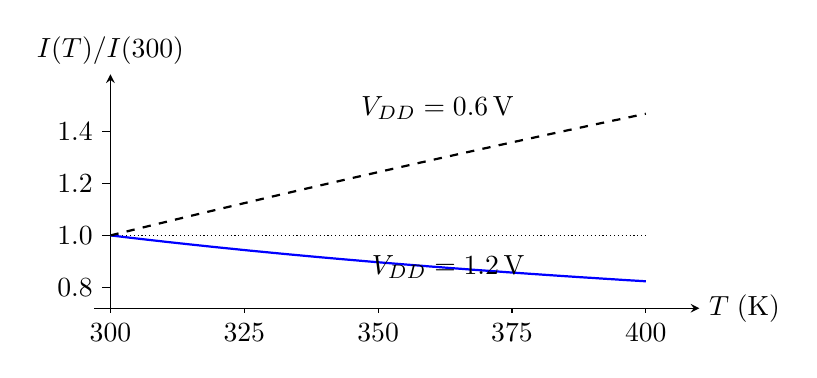
\begin{tikzpicture}[x=0.068cm,y=3.3cm,>=stealth]
\draw[->] (-3,0.72)--(110,0.72) node[right] {\(T\;(\mathrm{K})\)};
\draw[->] (0,0.72)--(0,1.62) node[above] {\(I(T)/I(300)\)};
\foreach \x/\t in {0/300,25/325,50/350,75/375,100/400}
 {\draw (\x,0.72)--(\x,0.70) node[below] {\(\t\)};}
\foreach \y in {0.8,1.0,1.2,1.4}
 {\draw (0,\y)--(-1.5,\y) node[left] {\(\y\)};}
\draw[densely dotted] (0,1)--(100,1);
\draw[thick,blue,domain=0:100,samples=70]
 plot (\x,{pow((300+\x)/300,-1.5)*pow((0.8+0.001*\x)/0.8,2)});
\draw[thick,dashed,domain=0:100,samples=70]
 plot (\x,{pow((300+\x)/300,-1.5)*pow((0.2+0.001*\x)/0.2,2)});
\node[anchor=west] at (47,0.88) {\(V_{DD}=1.2\,\mathrm{V}\)};
\node[anchor=west] at (45,1.49) {\(V_{DD}=0.6\,\mathrm{V}\)};
\end{tikzpicture}
\end{latin}
\caption{تغییر جریان نرمال‌شده برای پارامترهای فرضی مثال دما.
منحنی‌ها از رابطه \eqref{eq:temperature-current-ratio} محاسبه شده‌اند.}
\label{fig:temperature-on-ratio}
\end{figure}

\subsubsection*{معنای ضریب دمایی و استخراج شرط تغییر علامت}
مشتق \(\mathrm{d}I/\mathrm{d}T\)، نرخ تغییر جریان با تغییر کوچک
دماست. برای درک سهم عامل‌ها، می‌توان ابتدا تغییر نسبی را نوشت.
در مدل \eqref{eq:temperature-on-current}، جریان با \(\beta A^2\)
متناسب است که \(A(T)=V_{DD}-V_t(T)>0\) است. برای تغییر کوچک دما،
تغییر نسبی حاصل‌ضرب تقریباً برابر جمع تغییرهای نسبی عامل‌ها می‌شود
\begin{equation}
 \frac{\Delta I}{I}\approx
 \frac{\Delta\beta}{\beta}+2\frac{\Delta A}{A}.
 \label{eq:temperature-fractional-change}
\end{equation}
ضریب دو از مربع \(A\) می‌آید. مشتق دقیق همین بیان، با
\(\beta\propto T^{-k_\mu}\) و
\(\mathrm{d}A/\mathrm{d}T=k_{vt}\)، برابر است با
\begin{equation}
 \frac{1}{I}\frac{\mathrm{d}I}{\mathrm{d}T}
 =-\frac{k_\mu}{T}+\frac{2k_{vt}}{V_{DD}-V_t(T)}.
 \label{eq:temperature-coefficient}
\end{equation}
هر دو جمله واحد \(\unit{\per\kelvin}\) دارند. ضریب مثبت یعنی افزایش
جریان با گرم‌شدن در همسایگی همان نقطه. با صفرقراردادن طرف راست،
شرط توازن محلی به دست می‌آید
\begin{equation}
 V_{DD}-V_t(T)=\frac{2k_{vt}T}{k_\mu}.
 \label{eq:temperature-crossover}
\end{equation}
در \(\qty{300}{\kelvin}\) و با پارامترهای مثال، طرف راست
\(\qty{0.4}{\volt}\) است و توازن محلی در
\(V_{DD}=\qty{0.8}{\volt}\) رخ می‌دهد. این شرط، شیب جریان در یک
دمای مشخص را صفر می‌کند. برابری جریان در دو دمای با فاصله زیاد
باید مستقیماً از \eqref{eq:temperature-current-ratio} حل شود.

کتاب، رفتار معمول جریان روشن را در تغذیه بالا کاهشی توصیف می‌کند و
برای تغذیه پایین، افزایش جریان با دما را نیز مطرح می‌کند. بازه
تقریبی \(\qty{0.7}{\volt}\) تا \(\qty{1.1}{\volt}\) در متن کتاب به
نمونه‌های فناوری آن مرجع مربوط است. شکل‌های \secnum{۲.۲۳} و
\secnum{۲.۲۴} همان صفحه، تغییر شکل منحنی و کاهش معمول جریان روشن
را نمایش می‌دهند \cite[صفحه ۸۵]{weste}. تعیین نقطه تغییر علامت در
یک فناوری مشخص به مدل کامل همان فناوری نیاز دارد.

\subsubsection*{مثال آموزشی تغییر نشتی مطلق با دما}
در تمرین \secnum{۲.۱۰}، دو آستانه متفاوت در یک دمای مشترک مقایسه می‌شوند.
برای مقایسه دو دما، عامل پیش‌ضرب و ولتاژ حرارتی هم تغییر می‌کنند.
فرض کنید مدل \eqref{eq:leakage-subthreshold-model} با
\(V_{GS}=V_{SB}=0\)، \(V_{DS}=\qty{1}{\volt}\)، \(\eta=0\)،
\(n=1.4\) و همان \(\beta(T)\) و \(V_t(T)\) مثال دما به کار رود.
در این مدل آموزشی، \(n\)، هندسه و \(C_{\mathrm{ox}}\) ثابت‌اند.
اگر \(v_{T,i}=kT_i/q\) و
\(F_i=1-\exp(-V_{DS}/v_{T,i})\) باشند، تقسیم دو جریان می‌دهد
\begin{equation}
 \frac{I_2}{I_1}=
 \left(\frac{T_2}{T_1}\right)^{2-k_\mu}
 \exp\!\left[\frac{V_t(T_1)}{nv_{T,1}}
             -\frac{V_t(T_2)}{nv_{T,2}}\right]\frac{F_2}{F_1}.
 \label{eq:temperature-leakage-ratio}
\end{equation}
توان \(2-k_\mu\) از حاصل‌ضرب
\(\beta\propto T^{-k_\mu}\) و \(v_T^2\propto T^2\) در
\eqref{eq:leakage-current-prefactor} به دست آمده است.
ثابت تجربی \(e^{1.8}\) در نسبت حذف می‌شود.
با \(k/q\approx\qty{8.61733e-5}{\volt\per\kelvin}\)،
\(v_{T,1}\approx\qty{25.852}{\milli\volt}\) و
\(v_{T,2}\approx\qty{34.469}{\milli\volt}\) هستند.
در هر دو دما، \(V_{DS}/v_T>29\) و عامل \(F\) با دقت خوبی یک است.
جای‌گذاری \(V_t(300)=\qty{0.4}{\volt}\) و
\(V_t(400)=\qty{0.3}{\volt}\) نتیجه می‌دهد
\begin{equation}
 I_1\approx\qty{12.82}{\pico\ampere},\qquad
 I_2\approx\qty{1.864}{\nano\ampere},\qquad
 \frac{I_2}{I_1}\approx145.3.
 \label{eq:temperature-leakage-example}
\end{equation}
هر دو بایاس گیت زیر آستانه‌اند. رشد شدید در این مثال از تغییر عامل
نمایی ناشی می‌شود. مقدار واقعی رشد به پارامترها و بایاس وابسته است.
کتاب رشد شدید نشتی زیرآستانه، رشد آهسته‌تر \lr{BTBT} و وابستگی کم
نشتی گیت به دما را در محدوده بحث خود بیان می‌کند
\cite[صفحه ۸۵]{weste}. توان نشتی هر منبع از جریان همان منبع و
ولتاژ آن به دست می‌آید.

\subsubsection*{خنک‌کاری و سازگاری مدل میدان بحرانی}
کاهش دما معمولاً \lr{Mobility} را بیشتر و نشتی زیرآستانه را کمتر
می‌کند. مرجع، دفع گرما با همرفت، فن و \lr{Heat Sink} و روش‌های
قوی‌تر مانند خنک‌کاری آبی، سردکننده لایه‌نازک و نیتروژن مایع را
مطرح می‌کند. کاهش نشتی می‌تواند به انتخاب آستانه کمتر کمک کند.
متن همچنین افزایش پهنای ناحیه تخلیه و کاهش ظرفیت پیوند را در بحث
عملکرد دمای پایین بیان می‌کند \cite[صفحه ۸۶]{weste}.
این نتایج با فرض‌های بایاس و فناوری همان بحث تفسیر می‌شوند.

برای جهت تغییر \(E_c\)، رابطه \eqref{eq:critical-field} باید با هر
دو پارامتر بررسی شود. با تقریب‌های عددی همین بخش، داریم
\begin{equation}
 \frac{E_c(400)}{E_c(300)}
 =\frac{v_{\mathrm{sat}}(400)/v_{\mathrm{sat}}(300)}
        {\mu(400)/\mu(300)}
 \approx\frac{0.8}{0.6495}\approx1.232.
 \label{eq:temperature-critical-field}
\end{equation}
پس ترکیب این تقریب‌ها، میدان بحرانی بزرگ‌تر را در دمای بالاتر
می‌دهد. عبارت کیفی صفحه ۸۶ درباره وقوع اشباع سرعت در میدان‌های
بالاتر هنگام خنک‌کاری، با این انتخاب هم‌زمان پارامترها سازگار
نیست. در محاسبه این جزوه، جهت تغییر از نسبت
\(2v_{\mathrm{sat}}/\mu\) و داده‌های مدل تعیین می‌شود.

مرجع استفاده کوتاه‌مدت از اسپری سردکننده و دمنده هوای گرم را برای
تشخیص حساسیت دمایی مدار نیز بیان می‌کند و امکان آسیب ناشی از تغییر
ناگهانی دما به تراشه یا بسته‌بندی را یادآور می‌شود
\cite[صفحه ۸۶]{weste}. این توصیف، بخشی از محتوای مرجع است.

\clearpage
\subsection{وابستگی به هندسه}
\label{sec:geometry-dependence}
ابعاد ترسیم‌شده در \lr{Layout} با ابعاد مؤثر کانال تفاوت دارند.
کتاب و اسلایدها این تفاوت را با دو نوع اصلاح مدل می‌کنند
\cite[بخش \secnum{۲.۴.۶}، صفحه ۸۶]{weste}
\cite[اسلایدهای ۳۵ و ۳۶]{nonideal}. نمادهای
\(L_{\mathrm{drawn}},W_{\mathrm{drawn}}\) طول و عرض ترسیم‌شده‌اند.
اصلاح‌های علامت‌دار \(X_L,X_W\) تغییر ناشی از ساخت ماسک و فرایند
ساخت را نمایش می‌دهند. مثلاً \lr{Overetch} می‌تواند طول گیت را
کوتاه کند و \(X_L<0\) بدهد. پارامتر \(L_D\) سهم نفوذ جانبی از هر
طرف و \(W_D\) اصلاح کاهش عرض از هر لبه است.

\subsubsection*{استخراج ابعاد مؤثر و معنای ضریب دو}
پس از اصلاح ساخت، طول هندسی گیت
\(L_g=L_{\mathrm{drawn}}+X_L\) است. ناحیه‌های سورس و درین هر کدام
به اندازه \(L_D\) زیر گیت پیشروی می‌کنند. فاصله مؤثر عبور حامل‌ها
با کم‌کردن هر دو سهم به دست می‌آید. رابطه عرض نیز دو لبه دارد.
در نتیجه، رابطه \secnum{۲.۵۳} کتاب چنین نوشته می‌شود
\begin{align}
 L_{\mathrm{eff}}&=L_{\mathrm{drawn}}+X_L-2L_D,
 \label{eq:geometry-effective-length}\\
 W_{\mathrm{eff}}&=W_{\mathrm{drawn}}+X_W-2W_D.
 \label{eq:geometry-effective-width}
\end{align}
همه جمله‌ها واحد طول دارند. مقدارهای حاصل باید مثبت و در دامنه
اعتبار مدل فرایند باشند. شکل \ref{fig:geometry-length} سهم دو لبه
را به‌صورت شماتیک نمایش می‌دهد.
\begin{figure}[!htbp]
\centering
\begin{latin}
\PersianMathDigits
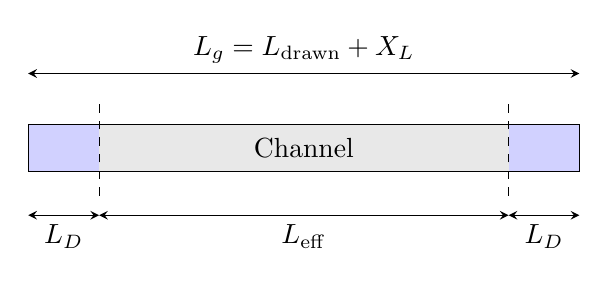
\begin{tikzpicture}[x=1cm,y=1cm,>=stealth]
\fill[gray!18] (0,0) rectangle (7,0.6);
\fill[blue!18] (0,0) rectangle (0.9,0.6);
\fill[blue!18] (6.1,0) rectangle (7,0.6);
\draw (0,0) rectangle (7,0.6);
\draw[dashed] (0.9,-0.3)--(0.9,0.9);
\draw[dashed] (6.1,-0.3)--(6.1,0.9);
\draw[<->] (0,1.25)--(7,1.25)
 node[midway,above] {\(L_g=L_{\mathrm{drawn}}+X_L\)};
\draw[<->] (0,-0.55)--(0.9,-0.55) node[midway,below] {\(L_D\)};
\draw[<->] (0.9,-0.55)--(6.1,-0.55)
 node[midway,below] {\(L_{\mathrm{eff}}\)};
\draw[<->] (6.1,-0.55)--(7,-0.55) node[midway,below] {\(L_D\)};
\node at (3.5,0.3) {Channel};
\end{tikzpicture}
\end{latin}
\caption{طرح آموزشی سهم نفوذ جانبی از دو سمت در طول مؤثر.
ابعاد شکل مقیاس فیزیکی ندارند.}
\label{fig:geometry-length}
\end{figure}

در بخش \ref{sec:clm}، نماد \(L_d\) با زیرنویس کوچک برای پیشروی
ناحیه تخلیه سمت درین در اثر بایاس به کار رفت. نماد \(L_D\) در این
بخش به نفوذ جانبی ناشی از ساخت مربوط است. هنگام ترکیب مدل‌ها، مرجع
طول و اصلاح بایاس را مشخص کنید تا یک کاهش طول دوبار وارد نشود.
در مدل \lr{CLM} ساده، \(\lambda\) اثر بایاس را در ضریب جریان
نمایش می‌دهد.

\subsubsection*{مثال آموزشی دوبرابرکردن طول و عرض ترسیم‌شده}
فرض کنید تمام ابعاد زیر برحسب نانومتر باشند و
\(X_L=X_W=-\qty{4}{\nano\metre}\)،
\(L_D=W_D=\qty{3}{\nano\metre}\).
برای افزاره مبنا با
\(L_{\mathrm{drawn}}=\qty{60}{\nano\metre}\) و
\(W_{\mathrm{drawn}}=\qty{120}{\nano\metre}\)، داریم
\[
 \begin{aligned}
 L_{\mathrm{eff}}&=60-4-2(3)=\qty{50}{\nano\metre},\\
 W_{\mathrm{eff}}&=120-4-2(3)=\qty{110}{\nano\metre}.
 \end{aligned}
\]
دوبرابرکردن طول ترسیم‌شده، طول مؤثر را به
\(120-4-6=\qty{110}{\nano\metre}\) می‌رساند. نسبت طول‌های مؤثر
\(110/50=2.2\) است. به همین ترتیب، دوبرابرکردن عرض ترسیم‌شده،
عرض مؤثر را \(\qty{230}{\nano\metre}\) می‌کند و نسبت عرض‌ها
\(230/110\approx2.091\) می‌شود.

برای محاسبه اثر هندسه به‌تنهایی، به‌طور آموزشی
\(k'=\mu C_{\mathrm{ox}}=\qty{200}{\micro\ampere\per\volt\squared}\)
و \(C_{\mathrm{ox}}=\qty{20}{\femto\farad\per\micro\metre\squared}\)
را ثابت فرض می‌کنیم. در تقریب مساحت مستطیلی کانال،
\begin{equation}
 \beta=k'\frac{W_{\mathrm{eff}}}{L_{\mathrm{eff}}},\qquad
 C_0=C_{\mathrm{ox}}W_{\mathrm{eff}}L_{\mathrm{eff}}.
 \label{eq:geometry-beta-capacitance}
\end{equation}
کمیت \(C_0\) مقیاس ظرفیت ذاتی گیت است. ظرفیت مؤثر هر پایانه به
ناحیه کاری و تقسیم بار وابسته است و ظرفیت‌های هم‌پوشانی و پیوند
نیز جداگانه مطرح‌اند. جدول \ref{tab:geometry-results} این محاسبه
هندسی را نشان می‌دهد.
\begin{table}[!htbp]
\centering
\small
\caption{نتایج هندسه فرضی با پارامترهای ماده ثابت.
طول‌ها برحسب \(\unit{\nano\metre}\) هستند.}
\label{tab:geometry-results}
\begin{tabularx}{\linewidth}{>{\raggedleft\arraybackslash}Xcccc}
\toprule
حالت & \(L_{\mathrm{eff}}\) & \(W_{\mathrm{eff}}\) &
\(\beta\)، \(\unit{\micro\ampere\per\volt\squared}\) &
\(C_0\)، \(\unit{\femto\farad}\)\\
\midrule
مبنا & \num{50} & \num{110} & \num{440} & \num{0.110}\\
طول ترسیم‌شده دوبرابر & \num{110} & \num{110} & \num{200} & \num{0.242}\\
عرض ترسیم‌شده دوبرابر & \num{50} & \num{230} & \num{920} & \num{0.230}\\
\bottomrule
\end{tabularx}
\end{table}
برای نمونه، \(\qty{50}{\nano\metre}=\qty{0.05}{\micro\metre}\)
و \(\qty{110}{\nano\metre}=\qty{0.11}{\micro\metre}\)، پس
مساحت مبنا \(\qty{0.0055}{\micro\metre\squared}\) است و
\(C_0=20(0.0055)=\qty{0.11}{\femto\farad}\) می‌شود.
در مدل مربعی با آستانه و بایاس ثابت، نسبت جریان برای تغییر طول
\(200/440\approx0.4545\) و برای تغییر عرض
\(920/440\approx2.091\) است.

در افزاره واقعی، هندسه می‌تواند آستانه را از راه اثر کانال کوتاه
و باریک نیز تغییر دهد. همچنین تغییر طول بر \lr{CLM} و
\lr{Velocity Saturation} اثر می‌گذارد. بنابراین، برای پیش‌بینی
جریان باید همه پارامترهای وابسته به هندسه را به‌روز کرد.
اسلاید ۳۶ افزایش آستانه و کاهش \lr{CLM} در کانال بلندتر را برای
روندهای مورد بحث دوره بیان می‌کند. نتیجه ساده \(I\propto1/L\)
به فرض ثابت‌بودن پارامترهای دیگر وابسته است
\cite[صفحه ۸۶]{weste}\cite[اسلاید ۳۶]{nonideal}.

\subsubsection*{هندسه یکسان و \lr{Matching}}
وقتی برابری یا نسبت دقیق جریان مهم است، کتاب استفاده از افزاره‌های
با طول و عرض یکسان را پیشنهاد می‌کند. برای نسبت‌های صحیح می‌توان
چند افزاره واحد یکسان را موازی کرد. مثلاً سه واحد موازی با بایاس‌های
پایانه‌ای یکسان، در مدل افزاره‌های یکسان سه برابر یک واحد جریان دارند.
هر واحد، همان اصلاح هندسی و آستانه واحد مبنا را تجربه می‌کند.

جهت‌گیری و محیط اطراف نیز بر ساخت اثر دارند. مرجع برای نمونه‌های
فرایندی کوچک‌تر از \(\qty{0.25}{\micro\metre}\)، اهمیت جهت‌گیری را
ذکر می‌کند. مقدار \lr{Polysilicon} مجاور می‌تواند سرعت حکاکی را
عوض کند. جهت‌گیری مشترک و \lr{Dummy Polysilicon} به یکنواختی محیط
کمک می‌کنند. چیدمان \lr{Interdigitated} یعنی درهم‌گذاری واحدهای
دو گروه، مانند ترتیب \lr{ABAB}، تا گروه‌ها محیط مکانی مشابه‌تری
ببینند. کتاب استفاده از آن را در صورت امکان مطرح می‌کند
\cite[صفحات ۸۶ و ۸۷]{weste}. انتخاب چیدمان واقعی تابع قواعد همان
فرایند و نوع خطای مورد کنترل است.

\subsubsection*{مکمل اسلایدها درباره \lr{PVT} و \lr{Process Corners}}
\label{sec:pvt-supplement}
اسلایدهای ۳۱ تا ۳۴، تغییر پارامترهای ساخت، تغذیه و دما را نیز
معرفی می‌کنند \cite{nonideal}. عبارت \lr{PVT} مخفف
\lr{Process, Voltage, Temperature} است. طول مؤثر، آستانه و ضخامت
عایق، مقادیر قطعی یکسان برای همه تراشه‌ها ندارند. تغذیه و دما نیز
در زمان و مکان تغییر می‌کنند. \lr{Corner} مجموعه‌ای مشخص از شرایط
مدل برای بررسی رفتار مدار است.

در قرارداد اسلایدها، \lr{T} به معنی \lr{Typical}، \lr{F} به معنی
\lr{Fast} و \lr{S} به معنی \lr{Slow} است. در مثال فرایندی اسلاید
۳۱، طول کوتاه‌تر، آستانه کمتر و عایق نازک‌تر به جریان قوی‌تر و
رفتار سریع‌تر کمک می‌کنند. پارامترهای \lr{nMOS} و \lr{pMOS} کاملاً
مستقل نیستند. دو حرف \lr{FS} یعنی \lr{nMOS} سریع و \lr{pMOS} کند،
و \lr{SF} حالت معکوس آن است. \lr{TT}، \lr{FF} و \lr{SS} نیز
به‌ترتیب حالت معمول و دو حالت هم‌جهت را نمایش می‌دهند.

اسلاید ۳۳ برای توصیف کامل‌تر، چهار حرف را به ترتیب
\lr{nMOS}، \lr{pMOS}، تغذیه و دما می‌نویسد. در قرارداد معمول همان
اسلایدها، تغذیه بالاتر و دمای پایین‌تر با حرف \lr{F} همراه‌اند.
جدول \ref{tab:pvt-environment} مقادیر نمونه اسلاید ۳۲ را بازنویسی
می‌کند. این مقادیر یک مثال درسی‌اند و باید برای هر فناوری از مدل
همان فناوری استفاده کرد. حرف \lr{T} در نام \lr{Corner} به معنی
حالت معمول است. نماد ریاضی \(T\) در روابط این جزوه دمای مطلق است.
\begin{table}[!htbp]
\centering
\caption{نمونه شرایط محیطی اسلاید ۳۲.}
\label{tab:pvt-environment}
\begin{tabular}{ccc}
\toprule
حالت & تغذیه، \(\unit{\volt}\) & دما، \(\unit{\degreeCelsius}\)\\
\midrule
\lr{F} & \num{1.98} & \num{0}\\
\lr{T} & \num{1.8} & \num{70}\\
\lr{S} & \num{1.62} & \num{125}\\
\bottomrule
\end{tabular}
\end{table}

در اسلاید ۳۴، مثال \lr{SSSS} برای بررسی زمان چرخه، \lr{FFFF}
برای توان و \lr{FFFS} برای نشتی زیرآستانه آمده است. برای نمونه،
\lr{FFFS} یعنی هر دو نوع ترانزیستور سریع، تغذیه بالا و دمای بالا.
آخرین حرف \lr{S} در اینجا همان دمای بالای جدول است.
گوشه توان \lr{FFFF} باید با مؤلفه توان مورد بررسی تفسیر شود.
توان دینامیکی از ظرفیت سوئیچ‌شونده، فعالیت، فرکانس و تغذیه اثر
می‌گیرد و توان نشتی نیز وابستگی دمایی خود را دارد. بنابراین، تعیین
بیشینه توان کل به مجموع مؤلفه‌ها و شرایط کار نیاز دارد.

حساسیت دمایی جریان در تغذیه پایین می‌تواند علامت عوض کند، چنان‌که
در \eqref{eq:temperature-coefficient} دیدیم. برای تعیین بدترین
تأخیر، باید دماهای مربوط به مدل بررسی شوند. همچنین بررسی
\lr{Corner}‌ها شواهدی درباره شرایط مدل‌شده فراهم می‌کند. پراکندگی
محلی و \lr{Mismatch} به مدل آماری مناسب خود نیاز دارند. این مکمل،
معنای قراردادهای اسلاید را برای خواندن تحلیل مدار روشن می‌کند.

% !TeX root = booklet-02.tex
\clearpage
\subsection{جمع‌بندی اثرهای غیرایده‌آل و کاربرد در مدار}
\label{sec:nonideal-summary}
بخش \secnum{۲.۴.۷} کتاب، نتیجه بحث را در پنج موضوع مدار جمع می‌کند
\cite[صفحات ۸۶ و ۸۷]{weste}. اسلاید ۳۰ نیز انتخاب تغذیه،
\lr{Logical Effort}، توان سکون، \lr{Pass Transistor} و دمای کار را
از کاربردهای این اثرها می‌شمارد \cite{nonideal}.

\subsubsection*{افت آستانه در عبور سطح منطقی}
وقتی \lr{nMOS} با گیت \(V_{DD}\) یک گره را به سمت سطح بالا شارژ
می‌کند، افزایش ولتاژ گره، \(V_{GS}\) را کاهش می‌دهد. در تقریب
آستانه ثابت، جریان هدایت قوی نزدیک
\(V_{\mathrm{out}}=V_{DD}-V_{tn}\) ضعیف می‌شود. در \lr{pMOS} که
سطح پایین را عبور می‌دهد، حد متناظر حدود \(|V_{tp}|\) بالای زمین
است. \lr{Body Effect} بزرگی افت آستانه را بیشتر می‌کند. وقتی آستانه
سهم بزرگی از تغذیه باشد، این افت برای سطح منطقی اهمیت بیشتری دارد.
در \lr{Transmission Gate}، یک \lr{nMOS} و یک \lr{pMOS} با کنترل
مکمل به‌صورت موازی قرار می‌گیرند. \lr{nMOS} عبور سطح پایین و
\lr{pMOS} عبور سطح بالا را تقویت می‌کند
\cite[بخش \secnum{۲.۴.۷}]{weste}. استخراج مشخصه انتقال و سطوح
منطقی این مدارها در بخش \secnum{۲.۵}، موضوع جزوه سوم است.

\subsubsection*{نشتی، توان سکون و نگهداری داده}
در \lr{Static CMOS} ایده‌آل، در حالت ماندگار مسیر هدایت بین تغذیه
و زمین قطع است. مدل واقعی مسیرهای نشتی بخش \ref{sec:leakage} را
دارد. در صورت تغذیه واحد و با قرارداد جریان مثبت دریافتی از منبع،
توان ماندگار \(P_{\mathrm{static}}=V_{DD}I_{DD}\) است.
برای چند منبع، سهم هر منبع از حاصل‌ضرب ولتاژ و جریان همان منبع
محاسبه می‌شود. جریان‌های شاخه‌ای باید با \lr{KCL} به جریان منبع
تبدیل شوند.

در گره‌ای که داده را به شکل بار ذخیره می‌کند، نشتی بار را جابه‌جا
می‌کند و ولتاژ گره تغییر می‌کند. برای ظرفیت ثابت،
\(\Delta Q=C\Delta V\) است. اگر جریان نشتی را در یک بازه تقریباً
ثابت فرض کنیم، \(|\Delta Q|\approx|I_{\mathrm{leak}}|\Delta t\)
و زمان رسیدن به تغییر ولتاژ مجاز تقریباً برابر می‌شود با
\begin{equation}
 \Delta t\approx\frac{C|\Delta V|}{|I_{\mathrm{leak}}|}.
 \label{eq:retention-time-estimate}
\end{equation}
واحد \(\mathrm{F}\,\mathrm{V}/\mathrm{A}=\mathrm{s}\) است.
این برآورد به ثابت‌بودن تقریبی ظرفیت و جریان تکیه دارد. در حالت
کلی، تغییر ولتاژ با جریان وابسته به ولتاژ و دما محاسبه می‌شود.
کتاب نیاز به \lr{Feedback} یا تجدید داده در ساختارهای ذخیره‌ساز را
از پیامدهای نشتی مطرح می‌کند. آستانه پایین، جریان روشن و سرعت را
تقویت می‌کند و آستانه بالا نشتی را کاهش می‌دهد. فرایندهای دارای
چند انتخاب آستانه از این وابستگی برای مسیرهای با نیازهای متفاوت
استفاده می‌کنند \cite[صفحه ۸۷]{weste}.

در روایت فناوری مرجع، نازک‌شدن عایق، نشتی تونلی گیت را مهم کرده
و استفاده از عایق‌های \lr{High-k} را برانگیخته است. همچنین شیب
زیرآستانه در نمونه‌های بحث کتاب در حدود
\(\qty{60}{\milli\volt}\) تا \(\qty{100}{\milli\volt}\) به ازای هر
دهه تغییر جریان است. رابطه \eqref{eq:leakage-subthreshold-slope}
وابستگی آن را به \(n\) و دما نشان می‌دهد
\cite[صفحات ۸۲ و ۸۷]{weste}.

\subsubsection*{انتخاب \lr{VDD} و بازده کاهش‌یابنده افزایش ولتاژ}
در مدل مربعی، جریان اشباع با مربع اضافه‌ولتاژ رشد می‌کند. با
\lr{Mobility Degradation} و \lr{Velocity Saturation}، رشد جریان
در بایاس بالا کندتر می‌شود. در نتیجه، افزایش تغذیه با بهبود جریان
کمتری نسبت به پیش‌بینی ساده مربعی همراه است. هم‌زمان، انرژی
سوئیچ‌کردن ظرفیت با \(V_{DD}^2\) رشد می‌کند. تنش عایق نازک و
کانال کوتاه نیز محدوده مجاز ولتاژ را محدود می‌کند
\cite[صفحه ۸۷]{weste}. مقدار مجاز ولتاژ و شرایط قابلیت اطمینان از
اطلاعات همان فناوری تعیین می‌شوند.

\subsubsection*{ترانزیستورهای سری، جریان و تأخیر}
در ساختار سری، ولتاژ کل بین چند افزاره تقسیم می‌شود. کاهش میدان
هر افزاره می‌تواند اثر \lr{Velocity Saturation} را کم کند. کتاب
بیان می‌کند که جریان دو \lr{nMOS} سری می‌تواند از نصف جریان یک
\lr{nMOS} با همان عرض و طول بیشتر باشد. این اثر برای \lr{nMOS}
با \lr{Mobility} بالاتر محسوس‌تر است
\cite[صفحه ۸۷]{weste}. در برآورد
\(t\approx C\Delta V/I\)، جریان بیشتر به زمان کوتاه‌تر برای
جابه‌جایی همان بار کمک می‌کند. مدل دقیق تأخیر به تغییر جریان و
ظرفیت طی گذار وابسته است.

تمرین‌های \secnum{۲.۲} و \secnum{۲.۳}، ساختار سری را با یک ترانزیستور طول \(2L\)
مقایسه می‌کنند. مثال آموزشی بخش \ref{sec:series-velocity-example}
مقایسه کتاب در جمع‌بندی را با یک ترانزیستور طول \(L\) انجام می‌دهد.
مشخص‌کردن افزاره مرجع و مدل، برای تفسیر نسبت جریان ضروری است.

\subsubsection*{تطبیق جریان و \lr{Matching}}
برای برابری رفتار، ابعاد، جهت‌گیری و محیط ساخت افزاره‌ها باید تا
حد امکان مشابه باشند. واحدهای موازی یکسان و درهم‌گذاری مناسب
می‌توانند به ساخت نسبت جریان کمک کنند. مثال بخش
\ref{sec:geometry-dependence} نشان داد که یک نسبت در ابعاد
ترسیم‌شده الزاماً همان نسبت را در ابعاد مؤثر ایجاد نمی‌کند
\cite[صفحات ۸۶ و ۸۷]{weste}.

\subsubsection*{مثال آموزشی جریان دو افزاره سری در مدل سرعت}
\label{sec:series-velocity-example}
دو \lr{nMOS} یکسان با گیت مشترک \(V_{DD}=\qty{1}{\volt}\)،
سورس پایین در زمین و درین بالا در \(\qty{1}{\volt}\) را در نظر
بگیرید. برای هر واحد فرض کنید
\(V_t=\qty{0.3}{\volt}\)، \(V_c=\qty{1}{\volt}\) و
\(\beta=\qty{400}{\micro\ampere\per\volt\squared}\) باشند.
اثر بدنه، \lr{DIBL} و \lr{CLM} در این مثال آموزشی حذف شده‌اند.
ولتاژ گره میانی را \(x\) می‌نامیم.
رابطه‌های \eqref{eq:high-field-linear} و
\eqref{eq:current-reduction-factor} را برای هر افزاره جداگانه به
کار می‌بریم. برای اختصار، اگر \(a=V_{GS}-V_t>0\) و \(d=V_{DS}\)
باشند، تابع جریان همین مدل را می‌نویسیم
\begin{equation}
 J(a,d)=
 \begin{cases}
 \displaystyle\beta\frac{ad-d^2/2}{1+d/V_c},
       &0\le d<\dfrac{aV_c}{a+V_c},\\[6pt]
 \displaystyle\frac{\beta a^2}{2(1+a/V_c)},
       &d\ge\dfrac{aV_c}{a+V_c}.
 \end{cases}
 \label{eq:series-velocity-function}
\end{equation}
برای افزاره پایین، \(a=0.7\) و \(d=x\) برحسب ولت‌اند.
برای افزاره بالا، \(a=0.7-x\) و \(d=1-x\) هستند. شرط برابری
جریان‌ها در گره میانی می‌شود
\begin{equation}
 J(0.7,x)=J(0.7-x,1-x).
 \label{eq:series-velocity-kcl}
\end{equation}
تابع‌ها با ولتاژ برحسب ولت و ضریب \(\beta\) داده‌شده ارزیابی
می‌شوند. ابتدا \(0<x<0.7\) را انتخاب می‌کنیم تا هر دو افزاره
روشن باشند. در \(x=\qty{0.1}{\volt}\)، جریان پایین
\(\qty{23.64}{\micro\ampere}\) و جریان بالا
\(\qty{45.00}{\micro\ampere}\) است. پس باید \(x\) افزایش یابد.
در \(x=\qty{0.2}{\volt}\)، این جریان‌ها به‌ترتیب
\(\qty{40.00}{\micro\ampere}\) و
\(\qty{33.33}{\micro\ampere}\) هستند. ریشه میان این دو مقدار است.
با نصف‌کردن مکرر بازه و انتخاب نیمه‌ای که اختلاف جریان در دو سر
آن تغییر علامت می‌دهد، نتیجه چنین به دست می‌آید
\begin{equation}
 x\approx\qty{0.17370}{\volt},\qquad
 I_{\mathrm{series}}\approx\qty{36.296}{\micro\ampere}.
 \label{eq:series-velocity-result}
\end{equation}
کنترل ناحیه کاری ضروری است. برای افزاره پایین، مرز اشباع
\(0.7/(1+0.7)\approx\qty{0.41176}{\volt}\) است و
\(x\) از آن کمتر است، پس شاخه \lr{Linear} انتخاب می‌شود.
برای افزاره بالا، اضافه‌ولتاژ
\(\qty{0.52630}{\volt}\)، ولتاژ درین و سورس
\(\qty{0.82630}{\volt}\) و مرز اشباع
\(\qty{0.34482}{\volt}\) است. پس افزاره بالا در اشباع است.

یک افزاره واحد طول \(L\) در همان بایاس کل، در اشباع قرار دارد و
جریان آن برابر است با
\begin{equation}
 I_{\mathrm{single}}=
 \frac{(400/2)(0.7)^2}{1+0.7/1}\,\unit{\micro\ampere}
 \approx\qty{57.647}{\micro\ampere}.
 \label{eq:series-velocity-reference}
\end{equation}
بنابراین، \(I_{\mathrm{series}}/I_{\mathrm{single}}\approx0.6296\)
است که از نصف بزرگ‌تر است. این مقدار، نتیجه پارامترها و فرض‌های
همین مثال است. برای افزودن اثر بدنه، باید آستانه افزاره بالا را
تابع \(x\) کرد و برابری جریان‌ها را دوباره حل کرد.

\subsubsection*{تمرین آموزشی نگهداری بار و پاسخ}
گرهی با ظرفیت ثابت \(\qty{10}{\femto\farad}\)، جریان نشتی تقریباً
ثابت \(\qty{1}{\nano\ampere}\) و تغییر ولتاژ مجاز
\(\qty{0.1}{\volt}\) فرض کنید. زمان برآوردی نگهداری بار چقدر است؟
با تبدیل واحدها و استفاده از \eqref{eq:retention-time-estimate}، زمان
برآوردی به دست می‌آید.
\[
 \Delta t=\frac{(10\times10^{-15})(0.1)}{10^{-9}}
 =\qty{1e-6}{\second}=\qty{1}{\micro\second}.
\]
اگر جریان در همان شرایط دو برابر شود و ظرفیت و حاشیه ولتاژ ثابت
بمانند، زمان به \(\qty{0.5}{\micro\second}\) کاهش می‌یابد.
برای نمونه واقعی با جریان متغیر، معادله تغییر بار باید با مدل
جریان همان گره حل شود.

\subsubsection*{راهنمای نهایی حل و نقشه پوشش منابع}
پیش از جای‌گذاری عددها، بایاس‌های پایانه‌ای، مدل مسئله و شرایط ثابت
را تعیین کنید. ابعاد مؤثر را با قرارداد مدل به کار ببرید. آستانه
متناسب با بدنه، درین، هندسه و دما را محاسبه کنید. سپس اضافه‌ولتاژ
و مرز ناحیه کاری را به دست آورید. در مدار چندترانزیستوری، ولتاژ
گره‌های داخلی از \lr{KCL} تعیین می‌شود. پس از حل، ناحیه کاری،
ریشه فیزیکی، واحدها، رفتار حدی و دامنه تقریب‌ها را بررسی کنید.
پارامترهای تجربی چند مدل باید با قرارداد یکسان ترکیب شوند.

جدول \ref{tab:booklet-two-coverage} مسیر بازگشت از موضوع به کتاب و
اسلاید را نشان می‌دهد. شماره‌های رابطه این جزوه مستقل از کتاب‌اند.
\begin{table}[!htbp]
\centering
\small
\caption{نقشه موضوعی بخش \secnum{۲.۴} کتاب و اسلایدهای \lr{Nonideal Transistor Theory}.}
\label{tab:booklet-two-coverage}
\begin{tabularx}{\linewidth}{c>{\raggedleft\arraybackslash}Xc}
\toprule
بخش کتاب & موضوع در همین جزوه & اسلاید\\
\midrule
\secnum{۲.۴.۱} & بخش \ref{sec:high-field}، میدان، سرعت و مدل توان & ۶ تا ۱۲\\
\secnum{۲.۴.۲} & بخش \ref{sec:clm}، \lr{CLM} و شیب خروجی & ۱۳ و ۱۴\\
\secnum{۲.۴.۳} & بخش \ref{sec:threshold-effects}، اثرهای آستانه & ۱۵ تا ۲۰\\
\secnum{۲.۴.۴} & بخش \ref{sec:leakage}، سه مسیر نشتی & ۲۱ تا ۲۸\\
\secnum{۲.۴.۵} & بخش \ref{sec:temperature-dependence}، رقابت اثرهای دما & ۲۹\\
\secnum{۲.۴.۶} & بخش \ref{sec:geometry-dependence}، ابعاد مؤثر و تطبیق & ۳۵ و ۳۶\\
\secnum{۲.۴.۷} & بخش \ref{sec:nonideal-summary}، پیامدهای مداری & ۳۰\\
مکمل دوره & \hyperref[sec:pvt-supplement]{مکمل \lr{PVT} و قراردادهای \lr{Corner}} & ۳۱ تا ۳۴\\
\bottomrule
\end{tabularx}
\end{table}

اسلایدهای ۳ تا ۵ مقدمه و مرور منحنی‌ها هستند و موضوع آن‌ها در مرور
پیش‌نیازها و آغاز بخش \ref{sec:nonideal-current} آمده است.
فهرست اسلاید ۳۷ با هفت تمرین سری نخست فصل دوم مطابقت دارد.
اثبات تمرین \secnum{۲.۶} در بخش \ref{sec:high-field}، حل \secnum{۲.۲} در بازسازی
مرجع مدار سری و حل \secnum{۲.۳} و \secnum{۲.۷} تا \secnum{۲.۹} در فصل تمرین‌های اثر آستانه
آمده است. فصل پایانی تمرین‌ها، مسئله \secnum{۲.۱۰} را با مقایسه مدل مربعی
و نشتی زیرآستانه حل می‌کند. این ترتیب، پیش‌نیاز هر تمرین را پیش از
حل آن فراهم می‌کند.

\BookletReview{notes/booklet-02/review-high-field}
\BookletReview{notes/booklet-02/threshold-exercises}
\BookletReview{notes/booklet-02/leakage-exercises}
